\section{Grouping things together...}
\textit{Symmetry} is one of the many things which both mathematicians and physicists crave to understand. And \textit{Group Theory} is a mathematically formal way of learning about these symmetries. The basic idea is to `cluster' the symmetries into some `groups' and then do all kind of nasty things to them. For that, first let us define the main hero of this act: a group.
\begin{definition}[Group]
    A group $g$ is a ordered pair $(G,*)$ where $G$ is a set and $*:G\times G\rightarrow G$ is a binary operation satisfying:
    \begin{itemize}
        \item \textbf{Associativity:} $g_1*(g_2*g_3) = (g_1*g_2)*g_3 \ \forall \ g_1,g_2,g_3\in G$
        \item \textbf{Identity:} There exists a unique $ e\in G$ such that $\forall \ g \in G, e*g = g*e = g$
        \item \textbf{Existence of Inverse:} For every $g\in G$, there exists $g^{-1}$ such that $g*g^{-1} = g^{-1}*g = e$
        \item \textbf{Closure:} $g*h\in G \ \forall \ g,h\in G$
    \end{itemize}
\end{definition}
A few points to note:
\begin{itemize}
    \item We sometimes (almost everytime) omit $*$ when the context is clear and just write $gh$ for $g*h$ where $g,h\in G$.
    \item Technically $(G,*)$ is called a group but when context is clear, the just simply refer to $G$ as the group.
    \item A group  $G$ is called \textit{Abelian} if the elements comute, that is, $\forall \ g_1,g_2 \in G \ g_1g_2 = g_2g_1$
\end{itemize}
Let us see some examples of groups, all of which can be checked to satisfy the properties specified in the definition:
\begin{enumerate}
    \item $(\re\backslash \{0\}, \times),(\re, +)$: the real numbers under multiplication\footnote{Note that under multiplication, no inverse exist for zero, so we exclude 0} and addition form a group. 
    \item $\mathrm{GL}(n,\re), \mathrm{GL}(n,\ce)$: the set of all invertible $n\times n$ matrices over $\re$ or $\ce$ field, form a \underline{g}eneral \underline{l}inear group under matrix multiplication. 
    \item $\mathrm{SL}(n,\re),\mathrm{SL}(n,\ce)$: the set of all invertible $n\times n$ matrices with determinant 1, over $\re$ or $\ce$ field, form a \underline{s}pecial \underline{l}inear group under matrix multiplication. 
    \item $\mathrm{O}(n),\mathrm{SO}(n)$: set of all orthogonal $n\times n$ matrices and orthogonal matrices with determinant 1 form \underline{o}rthogonal and \underline{s}pecial \underline{o}rthogonal group.
    \item $S_n$: the set of all permutations of $n$ objects form a group.  
    Permutation means arranging the same objects in some way, so basically it can be thought of as a bijection of a set onto itself. We represent these maps by $\pi$ such that $\pi : \{1,2,\ldots,n\}\rightarrow \{1,2,\ldots,n\}$ and 
$$   \pi \equiv 
\begin{pmatrix}
  1         & 2         & \cdots & n \\
  \pi(1) & \pi(2) & \cdots & \pi(n)
\end{pmatrix}$$
The above representation means that the first row, after the arrangement (acting on by map $pi$), changes to the second row. As an example, let us consider: 
$$\begin{pmatrix}
    \mathcolor{red}{1&2&3&4&5&6&7}\\
    \mathcolor{blue}{7&2&5&6&1&4&3}
\end{pmatrix}$$
The red elements are how the objects are initially there, blue are how the objects change place after permutation. Note that, under the map $\pi$, $1\rightarrow 7, 7\rightarrow 3, 3 \rightarrow 5, 5 \rightarrow 1$ and also $4\rightarrow 6, 6\rightarrow 4$ while 2 is mapped to 2 itself. This hints writing the thing in a cyclic structure, like $(1\ 7\ 3\ 5)(2)(4\ 6)$. We say $1,7,3,5$ form a \textit{4-cycle} while $4,6$ form a \textit{2-cycle}. 

\end{enumerate}
\subsection{Symmetries of the Equilateral Triangle}
This is one of the typical examples which is always mentioned in any group theory introduction, so as a reverence to the old-age custom, we include it too. To describe this, we will consider three actions on the triangle:
\begin{itemize}
    \item Leave it alone
    \item Rotate it by some angle
    \item Flip (reflect) it about some axis.
\end{itemize}
\begin{figure}[H]
    \centering 
    

\tikzset{every picture/.style={line width=0.75pt}} %set default line width to 0.75pt        

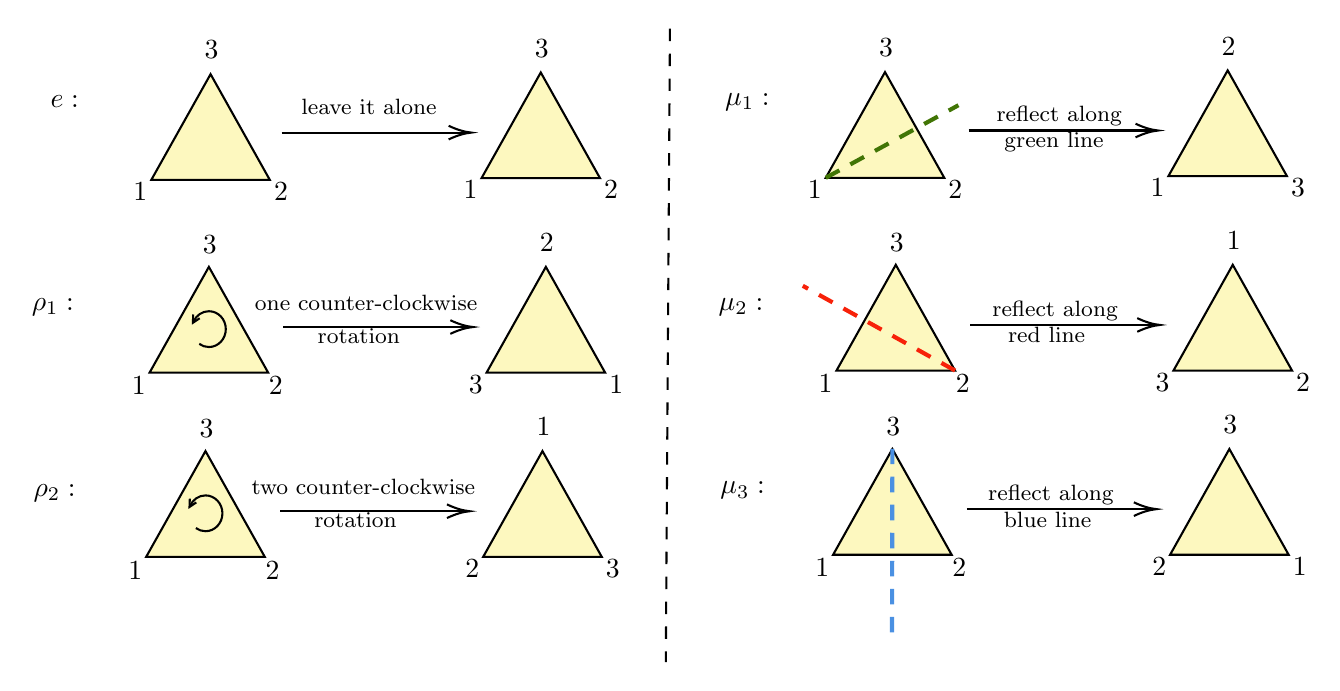
\begin{tikzpicture}[x=0.75pt,y=0.75pt,yscale=-1,xscale=1]
%uncomment if require: \path (0,370); %set diagram left start at 0, and has height of 370

%Shape: Triangle [id:dp770234789038906] 
\draw  [fill={rgb, 255:red, 250; green, 238; blue, 106 }  ,fill opacity=0.43 ] (99.67,41.9) -- (128.22,92.84) -- (71.11,92.84) -- cycle ;
%Shape: Triangle [id:dp3706336221489376] 
\draw  [fill={rgb, 255:red, 250; green, 238; blue, 106 }  ,fill opacity=0.43 ] (258.76,41.08) -- (287.31,92.02) -- (230.2,92.02) -- cycle ;

%Straight Lines [id:da4989662460487787] 
\draw    (133.93,70.05) -- (223.31,70.05) ;
\draw [shift={(225.31,70.05)}, rotate = 180] [color={rgb, 255:red, 0; green, 0; blue, 0 }  ][line width=0.75]    (10.93,-3.29) .. controls (6.95,-1.4) and (3.31,-0.3) .. (0,0) .. controls (3.31,0.3) and (6.95,1.4) .. (10.93,3.29)   ;
%Shape: Triangle [id:dp519914910955628] 
\draw  [fill={rgb, 255:red, 250; green, 238; blue, 106 }  ,fill opacity=0.43 ] (98.85,134.75) -- (127.41,185.69) -- (70.29,185.69) -- cycle ;
%Shape: Triangle [id:dp1396929998067723] 
\draw  [fill={rgb, 255:red, 250; green, 238; blue, 106 }  ,fill opacity=0.43 ] (261.21,134.75) -- (289.76,185.69) -- (232.65,185.69) -- cycle ;

%Straight Lines [id:da9582211177725937] 
\draw    (134.75,163.73) -- (224.12,163.73) ;
\draw [shift={(226.12,163.73)}, rotate = 180] [color={rgb, 255:red, 0; green, 0; blue, 0 }  ][line width=0.75]    (10.93,-3.29) .. controls (6.95,-1.4) and (3.31,-0.3) .. (0,0) .. controls (3.31,0.3) and (6.95,1.4) .. (10.93,3.29)   ;
%Shape: Arc [id:dp48627820726893056] 
\draw  [draw opacity=0] (91.49,161.01) .. controls (92.81,158.11) and (95.61,156.11) .. (98.85,156.11) .. controls (103.36,156.11) and (107.01,159.97) .. (107.01,164.74) .. controls (107.01,169.5) and (103.36,173.37) .. (98.85,173.37) .. controls (97.13,173.37) and (95.53,172.8) .. (94.21,171.84) -- (98.85,164.74) -- cycle ; \draw   (91.49,161.01) .. controls (92.81,158.11) and (95.61,156.11) .. (98.85,156.11) .. controls (103.36,156.11) and (107.01,159.97) .. (107.01,164.74) .. controls (107.01,169.5) and (103.36,173.37) .. (98.85,173.37) .. controls (97.13,173.37) and (95.53,172.8) .. (94.21,171.84) ;  
\draw   (94.43,159.51) -- (91.15,161.67) -- (91.31,157.69) ;

%Shape: Triangle [id:dp7800571980355699] 
\draw  [fill={rgb, 255:red, 250; green, 238; blue, 106 }  ,fill opacity=0.43 ] (97.22,223.49) -- (125.77,274.43) -- (68.66,274.43) -- cycle ;
%Shape: Triangle [id:dp26855524593503344] 
\draw  [fill={rgb, 255:red, 250; green, 238; blue, 106 }  ,fill opacity=0.43 ] (259.58,223.49) -- (288.13,274.43) -- (231.02,274.43) -- cycle ;

%Straight Lines [id:da20079967504625829] 
\draw    (133.12,252.47) -- (222.49,252.47) ;
\draw [shift={(224.49,252.47)}, rotate = 180] [color={rgb, 255:red, 0; green, 0; blue, 0 }  ][line width=0.75]    (10.93,-3.29) .. controls (6.95,-1.4) and (3.31,-0.3) .. (0,0) .. controls (3.31,0.3) and (6.95,1.4) .. (10.93,3.29)   ;
%Shape: Arc [id:dp7942405481223301] 
\draw  [draw opacity=0] (89.86,249.75) .. controls (91.17,246.85) and (93.97,244.85) .. (97.22,244.85) .. controls (101.72,244.85) and (105.38,248.72) .. (105.38,253.48) .. controls (105.38,258.25) and (101.72,262.11) .. (97.22,262.11) .. controls (95.5,262.11) and (93.9,261.54) .. (92.58,260.58) -- (97.22,253.48) -- cycle ; \draw   (89.86,249.75) .. controls (91.17,246.85) and (93.97,244.85) .. (97.22,244.85) .. controls (101.72,244.85) and (105.38,248.72) .. (105.38,253.48) .. controls (105.38,258.25) and (101.72,262.11) .. (97.22,262.11) .. controls (95.5,262.11) and (93.9,261.54) .. (92.58,260.58) ;  
\draw   (92.8,248.25) -- (89.52,250.41) -- (89.67,246.43) ;

%Straight Lines [id:da5406707716678466] 
\draw  [dash pattern={on 4.5pt off 4.5pt}]  (321,20) -- (319,325.18) ;
%Shape: Triangle [id:dp6812685355376344] 
\draw  [fill={rgb, 255:red, 250; green, 238; blue, 106 }  ,fill opacity=0.43 ] (424.61,40.9) -- (453.17,91.84) -- (396.06,91.84) -- cycle ;
%Shape: Triangle [id:dp08881040872765822] 
\draw  [fill={rgb, 255:red, 250; green, 238; blue, 106 }  ,fill opacity=0.43 ] (589.71,40.08) -- (618.26,91.02) -- (561.15,91.02) -- cycle ;

%Straight Lines [id:da3296001217074366] 
\draw    (464.88,69.05) -- (554.25,69.05) ;
\draw [shift={(556.25,69.05)}, rotate = 180] [color={rgb, 255:red, 0; green, 0; blue, 0 }  ][line width=0.75]    (10.93,-3.29) .. controls (6.95,-1.4) and (3.31,-0.3) .. (0,0) .. controls (3.31,0.3) and (6.95,1.4) .. (10.93,3.29)   ;
%Shape: Triangle [id:dp9818559862929847] 
\draw  [fill={rgb, 255:red, 250; green, 238; blue, 106 }  ,fill opacity=0.43 ] (429.8,133.75) -- (458.35,184.69) -- (401.24,184.69) -- cycle ;
%Shape: Triangle [id:dp5966925391786466] 
\draw  [fill={rgb, 255:red, 250; green, 238; blue, 106 }  ,fill opacity=0.43 ] (592.15,133.75) -- (620.71,184.69) -- (563.6,184.69) -- cycle ;

%Straight Lines [id:da7542950918096184] 
\draw    (465.69,162.73) -- (555.07,162.73) ;
\draw [shift={(557.07,162.73)}, rotate = 180] [color={rgb, 255:red, 0; green, 0; blue, 0 }  ][line width=0.75]    (10.93,-3.29) .. controls (6.95,-1.4) and (3.31,-0.3) .. (0,0) .. controls (3.31,0.3) and (6.95,1.4) .. (10.93,3.29)   ;
%Shape: Triangle [id:dp43284317392018445] 
\draw  [fill={rgb, 255:red, 250; green, 238; blue, 106 }  ,fill opacity=0.43 ] (428.16,222.49) -- (456.72,273.43) -- (399.61,273.43) -- cycle ;
%Shape: Triangle [id:dp8956773215716932] 
\draw  [fill={rgb, 255:red, 250; green, 238; blue, 106 }  ,fill opacity=0.43 ] (590.52,222.49) -- (619.08,273.43) -- (561.97,273.43) -- cycle ;

%Straight Lines [id:da21964377356872167] 
\draw    (464.06,251.47) -- (553.44,251.47) ;
\draw [shift={(555.44,251.47)}, rotate = 180] [color={rgb, 255:red, 0; green, 0; blue, 0 }  ][line width=0.75]    (10.93,-3.29) .. controls (6.95,-1.4) and (3.31,-0.3) .. (0,0) .. controls (3.31,0.3) and (6.95,1.4) .. (10.93,3.29)   ;
%Straight Lines [id:da8311353717920538] 
\draw [color={rgb, 255:red, 65; green, 117; blue, 5 }  ,draw opacity=1 ][line width=1.5]  [dash pattern={on 5.63pt off 4.5pt}]  (396.06,91.84) -- (460,56.87) ;
%Straight Lines [id:da06735691218924689] 
\draw [color={rgb, 255:red, 247; green, 33; blue, 9 }  ,draw opacity=1 ][line width=1.5]  [dash pattern={on 5.63pt off 4.5pt}]  (458.35,184.69) -- (385,143.87) ;
%Straight Lines [id:da04188916516791419] 
\draw [color={rgb, 255:red, 74; green, 144; blue, 226 }  ,draw opacity=1 ][line width=1.5]  [dash pattern={on 5.63pt off 4.5pt}]  (428,310.87) -- (428.16,222.49) ;

% Text Node
\draw (61.03,92.64) node [anchor=north west][inner sep=0.75pt]    {$1$};
% Text Node
\draw (128.75,92.64) node [anchor=north west][inner sep=0.75pt]    {$2$};
% Text Node
\draw (95.3,24.44) node [anchor=north west][inner sep=0.75pt]    {$3$};
% Text Node
\draw (141.9,52.62) node [anchor=north west][inner sep=0.75pt]   [align=left] {{\footnotesize leave it alone}};
% Text Node
\draw (220.12,91.82) node [anchor=north west][inner sep=0.75pt]    {$1$};
% Text Node
\draw (287.84,91.82) node [anchor=north west][inner sep=0.75pt]    {$2$};
% Text Node
\draw (254.39,23.62) node [anchor=north west][inner sep=0.75pt]    {$3$};
% Text Node
\draw (60.22,186.31) node [anchor=north west][inner sep=0.75pt]    {$1$};
% Text Node
\draw (126.3,186.31) node [anchor=north west][inner sep=0.75pt]    {$2$};
% Text Node
\draw (94.48,118.11) node [anchor=north west][inner sep=0.75pt]    {$3$};
% Text Node
\draw (119.54,146.86) node [anchor=north west][inner sep=0.75pt]   [align=left] {{\footnotesize one counter-clockwise}\\{\footnotesize  \ \ \ \ \ \ \ \ rotation}};
% Text Node
\draw (256.84,117.29) node [anchor=north west][inner sep=0.75pt]    {$2$};
% Text Node
\draw (290.29,185.49) node [anchor=north west][inner sep=0.75pt]    {$1$};
% Text Node
\draw (222.57,185.49) node [anchor=north west][inner sep=0.75pt]    {$3$};
% Text Node
\draw (58.58,275.05) node [anchor=north west][inner sep=0.75pt]    {$1$};
% Text Node
\draw (124.67,275.05) node [anchor=north west][inner sep=0.75pt]    {$2$};
% Text Node
\draw (92.85,206.85) node [anchor=north west][inner sep=0.75pt]    {$3$};
% Text Node
\draw (117.91,235.6) node [anchor=north west][inner sep=0.75pt]   [align=left] {{\footnotesize two counter-clockwise}\\{\footnotesize  \ \ \ \ \ \ \ \ rotation}};
% Text Node
\draw (255.21,206.03) node [anchor=north west][inner sep=0.75pt]    {$1$};
% Text Node
\draw (288.66,274.23) node [anchor=north west][inner sep=0.75pt]    {$3$};
% Text Node
\draw (220.94,274.23) node [anchor=north west][inner sep=0.75pt]    {$2$};
% Text Node
\draw (21.13,50.73) node [anchor=north west][inner sep=0.75pt]    {$e:$};
% Text Node
\draw (12.05,148.33) node [anchor=north west][inner sep=0.75pt]    {$\rho _{1} :$};
% Text Node
\draw (12.87,237.9) node [anchor=north west][inner sep=0.75pt]    {$\rho _{2} :$};
% Text Node
\draw (385.98,91.64) node [anchor=north west][inner sep=0.75pt]    {$1$};
% Text Node
\draw (453.69,91.64) node [anchor=north west][inner sep=0.75pt]    {$2$};
% Text Node
\draw (420.24,23.44) node [anchor=north west][inner sep=0.75pt]    {$3$};
% Text Node
\draw (476.84,55.62) node [anchor=north west][inner sep=0.75pt]  [font=\footnotesize] [align=left] {reflect along \\ \ green line};
% Text Node
\draw (391.16,185.31) node [anchor=north west][inner sep=0.75pt]    {$1$};
% Text Node
\draw (457.25,185.31) node [anchor=north west][inner sep=0.75pt]    {$2$};
% Text Node
\draw (425.43,117.11) node [anchor=north west][inner sep=0.75pt]    {$3$};
% Text Node
\draw (389.53,274.05) node [anchor=north west][inner sep=0.75pt]    {$1$};
% Text Node
\draw (455.61,274.05) node [anchor=north west][inner sep=0.75pt]    {$2$};
% Text Node
\draw (423.8,205.85) node [anchor=north west][inner sep=0.75pt]    {$3$};
% Text Node
\draw (346.08,49.73) node [anchor=north west][inner sep=0.75pt]    {$\mu _{1} :$};
% Text Node
\draw (343,148.33) node [anchor=north west][inner sep=0.75pt]    {$\mu _{2} :$};
% Text Node
\draw (343.82,236.9) node [anchor=north west][inner sep=0.75pt]    {$\mu _{3} :$};
% Text Node
\draw (586.15,205.03) node [anchor=north west][inner sep=0.75pt]    {$3$};
% Text Node
\draw (619.6,273.23) node [anchor=north west][inner sep=0.75pt]    {$1$};
% Text Node
\draw (551.89,273.23) node [anchor=north west][inner sep=0.75pt]    {$2$};
% Text Node
\draw (587.78,116.29) node [anchor=north west][inner sep=0.75pt]    {$1$};
% Text Node
\draw (621.24,184.49) node [anchor=north west][inner sep=0.75pt]    {$2$};
% Text Node
\draw (553.52,184.49) node [anchor=north west][inner sep=0.75pt]    {$3$};
% Text Node
\draw (585.34,22.62) node [anchor=north west][inner sep=0.75pt]    {$2$};
% Text Node
\draw (618.79,90.82) node [anchor=north west][inner sep=0.75pt]    {$3$};
% Text Node
\draw (551.07,90.82) node [anchor=north west][inner sep=0.75pt]    {$1$};
% Text Node
\draw (474.84,149.62) node [anchor=north west][inner sep=0.75pt]  [font=\footnotesize] [align=left] {reflect along \\ \ \ red line};
% Text Node
\draw (472.84,238.62) node [anchor=north west][inner sep=0.75pt]  [font=\footnotesize] [align=left] {reflect along \\ \ \ blue line};


\end{tikzpicture}

    \caption{Diagram showing the different actions of reflection and rotations to the equilateral triangle.}
\end{figure}
Okay, so these six actions form a group for the symmetries of an equilateral triangle. To check that, we can try to form the multiplication table for these operations, which is a table demonstrating the result of the composition of the elements with each other. The table looks like something like this:
\begin{table}[H]
\centering
\renewcommand{\arraystretch}{1.0} % optional: adds vertical spacing
\begin{tabular}{|
    >{\centering\arraybackslash}p{0.03\textwidth}|
    >{\centering\arraybackslash}p{0.03\textwidth}|
    >{\centering\arraybackslash}p{0.03\textwidth}|
    >{\centering\arraybackslash}p{0.03\textwidth}|
    >{\centering\arraybackslash}p{0.03\textwidth}|
    >{\centering\arraybackslash}p{0.03\textwidth}|
    >{\centering\arraybackslash}p{0.03\textwidth}|
    }
\hline
\text{\Large $*$} & $e$ & $\rho_1$ & $\rho_2$ & $\mu_1$ & $\mu_2$ & $\mu_3$ \\
\hline
$e $     &   &   &   &   &   &   \\
\hline
$\rho_1$ &   &   &   &   &   &   \\
\hline
$\rho_2$ &   &   &   &   &   &   \\
\hline
$\mu_1$  &   &   &   &   &   &   \\
\hline
$\mu_2$  &   &   &   &   &   &   \\
\hline
$\mu_3$  &   &   &   &   &   &   \\
\hline
\end{tabular}
\end{table}
\noindent
Now, note the following things: First, the first row and first column will be filled as it is, since acting with identity does not change anything. Second, $\rho_1^2 \equiv \rho_2$ (since it is how we defined it).\\[0.2cm] Also, note that rotations will commute with themselves and one anti-clockwise rotation is rotation by $120^\circ$, so accordingly $\rho_1 \equiv 120^\circ$, $\rho_2\equiv 240^\circ$ and hence $\rho_2\rho_1 = \rho_1\rho_2 \equiv 360^\circ \equiv e, \rho_2^2 \equiv 480^\circ \equiv 120^\circ \equiv \rho_1$.\\[0.2cm]
Also, reflecting along the same line twice will result in the initial configuration, so $\mu_i^2 \equiv e \ \forall \ i $ Let us now fill the table with these information:

\begin{table}[H]
\centering
\renewcommand{\arraystretch}{1.6} % optional: adds vertical spacing
\begin{tabular}{|
    >{\centering\arraybackslash}p{0.06\textwidth}|
    >{\centering\arraybackslash}p{0.06\textwidth}|
    >{\centering\arraybackslash}p{0.06\textwidth}|
    >{\centering\arraybackslash}p{0.06\textwidth}|
    >{\centering\arraybackslash}p{0.06\textwidth}|
    >{\centering\arraybackslash}p{0.06\textwidth}|
    >{\centering\arraybackslash}p{0.06\textwidth}|
    }
\hline
\text{\Large $*$} & $e$ & $\rho_1$ & $\rho_2$ & $\mu_1$ & $\mu_2$ & $\mu_3$ \\
\hline
$e $   &  $e$ & $\rho_1$ & $\rho_2$ & $\mu_1$ & $\mu_2$ & $\mu_3$   \\
\hline
$\rho_1$ & $\rho_1$   &  $\rho_2$  &  $e$ &   &   &   \\
\hline
$\rho_2$ &  $\rho_2$  & $e$  &   $\rho_1$ &   &   &   \\
\hline
$\mu_1$  & $\mu_1$   &   &   &$e$   &   &   \\
\hline
$\mu_2$  & $\mu_2$  &   &   &   & $e$  &   \\
\hline
$\mu_3$  &  $\mu_3$ &   &   &   &   &  $e$ \\
\hline
\end{tabular}
\end{table}
\noindent
Now there are the non-intuitive actions left, combining rotation with reflections and reflections with reflections. Let us see these actions. We have to be careful with the following :
\begin{itemize}
    \item $ab$ means $b$ is acted first and then $a$. 
    \item When taking reflections, we should take them along the axes specified initially, not based on the current position of the index. So, $\mu_2$ does not mean taking reflection along the axis passing through the vertex with `2' on it. $\mu_2$ is taking reflection from the bottom-right vertex of the triangle, irrespective of what index is there on the vertex. 
\end{itemize}
\begin{figure}[H]
    \centering
    

\tikzset{every picture/.style={line width=0.75pt}} %set default line width to 0.75pt        

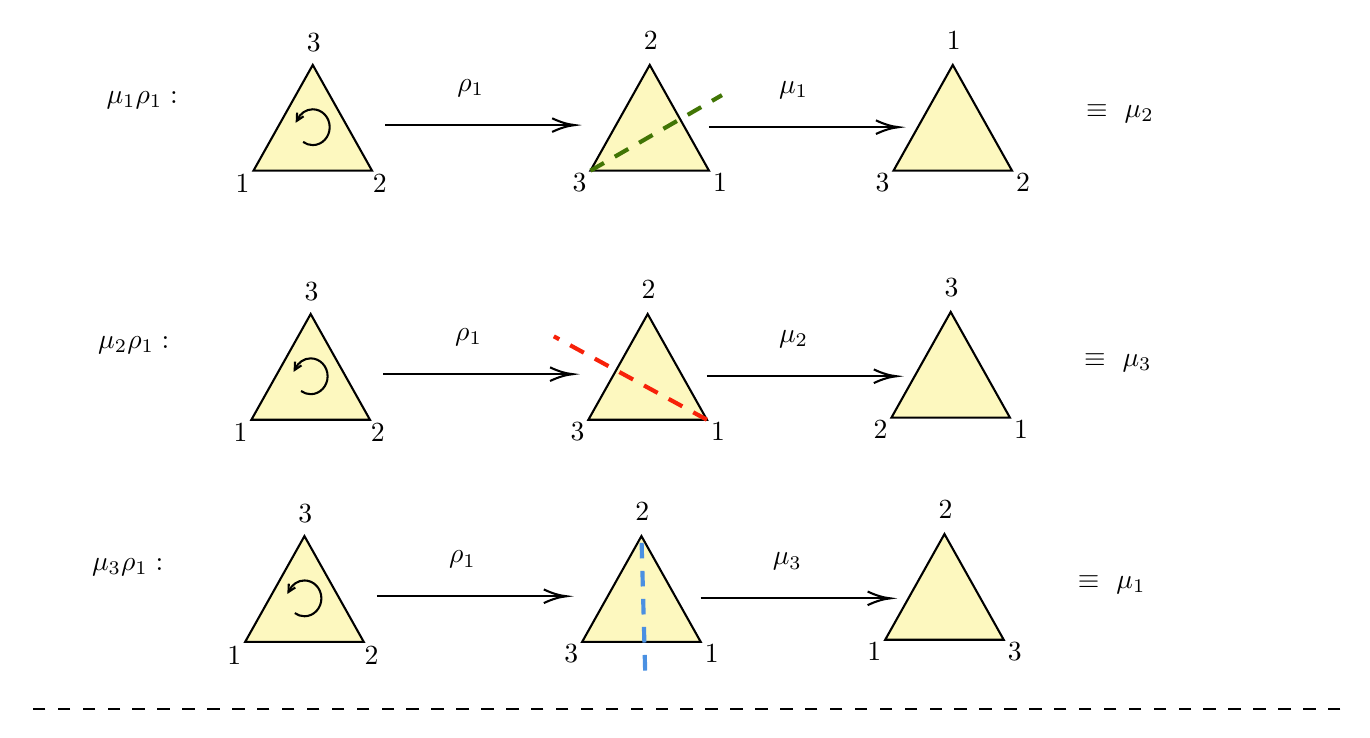
\begin{tikzpicture}[x=0.75pt,y=0.75pt,yscale=-1,xscale=1]
%uncomment if require: \path (0,350); %set diagram left start at 0, and has height of 350

%Shape: Triangle [id:dp18279766660658403] 
\draw  [fill={rgb, 255:red, 250; green, 238; blue, 106 }  ,fill opacity=0.43 ] (141.85,151.75) -- (170.41,202.69) -- (113.29,202.69) -- cycle ;
%Shape: Triangle [id:dp4197310425493971] 
\draw  [fill={rgb, 255:red, 250; green, 238; blue, 106 }  ,fill opacity=0.43 ] (304.21,151.75) -- (332.76,202.69) -- (275.65,202.69) -- cycle ;

%Straight Lines [id:da930520097755943] 
\draw    (176.75,180.73) -- (266.12,180.73) ;
\draw [shift={(268.12,180.73)}, rotate = 180] [color={rgb, 255:red, 0; green, 0; blue, 0 }  ][line width=0.75]    (10.93,-3.29) .. controls (6.95,-1.4) and (3.31,-0.3) .. (0,0) .. controls (3.31,0.3) and (6.95,1.4) .. (10.93,3.29)   ;
%Shape: Arc [id:dp215844960607804] 
\draw  [draw opacity=0] (134.49,178.01) .. controls (135.81,175.11) and (138.61,173.11) .. (141.85,173.11) .. controls (146.36,173.11) and (150.01,176.97) .. (150.01,181.74) .. controls (150.01,186.5) and (146.36,190.37) .. (141.85,190.37) .. controls (140.13,190.37) and (138.53,189.8) .. (137.21,188.84) -- (141.85,181.74) -- cycle ; \draw   (134.49,178.01) .. controls (135.81,175.11) and (138.61,173.11) .. (141.85,173.11) .. controls (146.36,173.11) and (150.01,176.97) .. (150.01,181.74) .. controls (150.01,186.5) and (146.36,190.37) .. (141.85,190.37) .. controls (140.13,190.37) and (138.53,189.8) .. (137.21,188.84) ;  
\draw   (137.43,176.51) -- (134.15,178.67) -- (134.31,174.69) ;

%Straight Lines [id:da5632790371547318] 
\draw [color={rgb, 255:red, 247; green, 33; blue, 9 }  ,draw opacity=1 ][line width=1.5]  [dash pattern={on 5.63pt off 4.5pt}]  (332.76,202.69) -- (259,162.5) ;
%Shape: Triangle [id:dp6887834214805665] 
\draw  [fill={rgb, 255:red, 250; green, 238; blue, 106 }  ,fill opacity=0.43 ] (450.21,150.75) -- (478.76,201.69) -- (421.65,201.69) -- cycle ;

%Straight Lines [id:da8273926927450299] 
\draw    (332.75,181.73) -- (422.12,181.73) ;
\draw [shift={(424.12,181.73)}, rotate = 180] [color={rgb, 255:red, 0; green, 0; blue, 0 }  ][line width=0.75]    (10.93,-3.29) .. controls (6.95,-1.4) and (3.31,-0.3) .. (0,0) .. controls (3.31,0.3) and (6.95,1.4) .. (10.93,3.29)   ;
%Shape: Triangle [id:dp13836286231856076] 
\draw  [fill={rgb, 255:red, 250; green, 238; blue, 106 }  ,fill opacity=0.43 ] (142.85,31.75) -- (171.41,82.69) -- (114.29,82.69) -- cycle ;
%Shape: Triangle [id:dp9253244528119978] 
\draw  [fill={rgb, 255:red, 250; green, 238; blue, 106 }  ,fill opacity=0.43 ] (305.21,31.75) -- (333.76,82.69) -- (276.65,82.69) -- cycle ;

%Straight Lines [id:da23996092927188062] 
\draw    (177.75,60.73) -- (267.12,60.73) ;
\draw [shift={(269.12,60.73)}, rotate = 180] [color={rgb, 255:red, 0; green, 0; blue, 0 }  ][line width=0.75]    (10.93,-3.29) .. controls (6.95,-1.4) and (3.31,-0.3) .. (0,0) .. controls (3.31,0.3) and (6.95,1.4) .. (10.93,3.29)   ;
%Shape: Arc [id:dp8896128197930823] 
\draw  [draw opacity=0] (135.49,58.01) .. controls (136.81,55.11) and (139.61,53.11) .. (142.85,53.11) .. controls (147.36,53.11) and (151.01,56.97) .. (151.01,61.74) .. controls (151.01,66.5) and (147.36,70.37) .. (142.85,70.37) .. controls (141.13,70.37) and (139.53,69.8) .. (138.21,68.84) -- (142.85,61.74) -- cycle ; \draw   (135.49,58.01) .. controls (136.81,55.11) and (139.61,53.11) .. (142.85,53.11) .. controls (147.36,53.11) and (151.01,56.97) .. (151.01,61.74) .. controls (151.01,66.5) and (147.36,70.37) .. (142.85,70.37) .. controls (141.13,70.37) and (139.53,69.8) .. (138.21,68.84) ;  
\draw   (138.43,56.51) -- (135.15,58.67) -- (135.31,54.69) ;

%Shape: Triangle [id:dp795571423848466] 
\draw  [fill={rgb, 255:red, 250; green, 238; blue, 106 }  ,fill opacity=0.43 ] (451.21,31.75) -- (479.76,82.69) -- (422.65,82.69) -- cycle ;

%Straight Lines [id:da9572482179097236] 
\draw    (333.75,61.73) -- (423.12,61.73) ;
\draw [shift={(425.12,61.73)}, rotate = 180] [color={rgb, 255:red, 0; green, 0; blue, 0 }  ][line width=0.75]    (10.93,-3.29) .. controls (6.95,-1.4) and (3.31,-0.3) .. (0,0) .. controls (3.31,0.3) and (6.95,1.4) .. (10.93,3.29)   ;
%Straight Lines [id:da20730078002652064] 
\draw [color={rgb, 255:red, 65; green, 117; blue, 5 }  ,draw opacity=1 ][line width=1.5]  [dash pattern={on 5.63pt off 4.5pt}]  (276.65,82.69) -- (340,46.3) ;
%Shape: Triangle [id:dp26218350538367785] 
\draw  [fill={rgb, 255:red, 250; green, 238; blue, 106 }  ,fill opacity=0.43 ] (138.85,258.75) -- (167.41,309.69) -- (110.29,309.69) -- cycle ;
%Shape: Triangle [id:dp7257387830462504] 
\draw  [fill={rgb, 255:red, 250; green, 238; blue, 106 }  ,fill opacity=0.43 ] (301.21,258.75) -- (329.76,309.69) -- (272.65,309.69) -- cycle ;

%Straight Lines [id:da43043420907131935] 
\draw    (173.75,287.73) -- (263.12,287.73) ;
\draw [shift={(265.12,287.73)}, rotate = 180] [color={rgb, 255:red, 0; green, 0; blue, 0 }  ][line width=0.75]    (10.93,-3.29) .. controls (6.95,-1.4) and (3.31,-0.3) .. (0,0) .. controls (3.31,0.3) and (6.95,1.4) .. (10.93,3.29)   ;
%Shape: Arc [id:dp2345241317556913] 
\draw  [draw opacity=0] (131.49,285.01) .. controls (132.81,282.11) and (135.61,280.11) .. (138.85,280.11) .. controls (143.36,280.11) and (147.01,283.97) .. (147.01,288.74) .. controls (147.01,293.5) and (143.36,297.37) .. (138.85,297.37) .. controls (137.13,297.37) and (135.53,296.8) .. (134.21,295.84) -- (138.85,288.74) -- cycle ; \draw   (131.49,285.01) .. controls (132.81,282.11) and (135.61,280.11) .. (138.85,280.11) .. controls (143.36,280.11) and (147.01,283.97) .. (147.01,288.74) .. controls (147.01,293.5) and (143.36,297.37) .. (138.85,297.37) .. controls (137.13,297.37) and (135.53,296.8) .. (134.21,295.84) ;  
\draw   (134.43,283.51) -- (131.15,285.67) -- (131.31,281.69) ;

%Shape: Triangle [id:dp1407114381804121] 
\draw  [fill={rgb, 255:red, 250; green, 238; blue, 106 }  ,fill opacity=0.43 ] (447.21,257.75) -- (475.76,308.69) -- (418.65,308.69) -- cycle ;

%Straight Lines [id:da39649581628084885] 
\draw    (329.75,288.73) -- (419.12,288.73) ;
\draw [shift={(421.12,288.73)}, rotate = 180] [color={rgb, 255:red, 0; green, 0; blue, 0 }  ][line width=0.75]    (10.93,-3.29) .. controls (6.95,-1.4) and (3.31,-0.3) .. (0,0) .. controls (3.31,0.3) and (6.95,1.4) .. (10.93,3.29)   ;
%Straight Lines [id:da39217256062402506] 
\draw [color={rgb, 255:red, 74; green, 144; blue, 226 }  ,draw opacity=1 ][line width=1.5]  [dash pattern={on 5.63pt off 4.5pt}]  (303,323.52) -- (301.21,258.75) ;
%Straight Lines [id:da04582911895669162] 
\draw  [dash pattern={on 4.5pt off 4.5pt}]  (638,341.9) -- (6,341.9) ;

% Text Node
\draw (103.22,203.31) node [anchor=north west][inner sep=0.75pt]    {$1$};
% Text Node
\draw (169.3,203.31) node [anchor=north west][inner sep=0.75pt]    {$2$};
% Text Node
\draw (137.48,135.11) node [anchor=north west][inner sep=0.75pt]    {$3$};
% Text Node
\draw (299.84,134.29) node [anchor=north west][inner sep=0.75pt]    {$2$};
% Text Node
\draw (333.29,202.49) node [anchor=north west][inner sep=0.75pt]    {$1$};
% Text Node
\draw (265.57,202.49) node [anchor=north west][inner sep=0.75pt]    {$3$};
% Text Node
\draw (210,157.4) node [anchor=north west][inner sep=0.75pt]    {$\rho _{1}$};
% Text Node
\draw (445.84,133.29) node [anchor=north west][inner sep=0.75pt]    {$3$};
% Text Node
\draw (479.29,201.49) node [anchor=north west][inner sep=0.75pt]    {$1$};
% Text Node
\draw (411.57,201.49) node [anchor=north west][inner sep=0.75pt]    {$2$};
% Text Node
\draw (366,158.4) node [anchor=north west][inner sep=0.75pt]    {$\mu _{2}$};
% Text Node
\draw (513,169.4) node [anchor=north west][inner sep=0.75pt]    {$\equiv \ \mu _{3}$};
% Text Node
\draw (104.22,83.31) node [anchor=north west][inner sep=0.75pt]    {$1$};
% Text Node
\draw (170.3,83.31) node [anchor=north west][inner sep=0.75pt]    {$2$};
% Text Node
\draw (138.48,15.11) node [anchor=north west][inner sep=0.75pt]    {$3$};
% Text Node
\draw (211,37.4) node [anchor=north west][inner sep=0.75pt]    {$\rho _{1}$};
% Text Node
\draw (366,38.4) node [anchor=north west][inner sep=0.75pt]    {$\mu _{1}$};
% Text Node
\draw (514,49.4) node [anchor=north west][inner sep=0.75pt]    {$\equiv \ \mu _{2}$};
% Text Node
\draw (446.84,14.29) node [anchor=north west][inner sep=0.75pt]    {$1$};
% Text Node
\draw (480.29,82.49) node [anchor=north west][inner sep=0.75pt]    {$2$};
% Text Node
\draw (412.57,82.49) node [anchor=north west][inner sep=0.75pt]    {$3$};
% Text Node
\draw (300.84,14.29) node [anchor=north west][inner sep=0.75pt]    {$2$};
% Text Node
\draw (334.29,82.49) node [anchor=north west][inner sep=0.75pt]    {$1$};
% Text Node
\draw (266.57,82.49) node [anchor=north west][inner sep=0.75pt]    {$3$};
% Text Node
\draw (42,43.12) node [anchor=north west][inner sep=0.75pt]    {$\mu _{1} \rho _{1} :$};
% Text Node
\draw (38,161.12) node [anchor=north west][inner sep=0.75pt]    {$\mu _{2} \rho _{1} :$};
% Text Node
\draw (100.22,310.31) node [anchor=north west][inner sep=0.75pt]    {$1$};
% Text Node
\draw (166.3,310.31) node [anchor=north west][inner sep=0.75pt]    {$2$};
% Text Node
\draw (134.48,242.11) node [anchor=north west][inner sep=0.75pt]    {$3$};
% Text Node
\draw (207,264.4) node [anchor=north west][inner sep=0.75pt]    {$\rho _{1}$};
% Text Node
\draw (363,265.4) node [anchor=north west][inner sep=0.75pt]    {$\mu _{3}$};
% Text Node
\draw (510,276.4) node [anchor=north west][inner sep=0.75pt]    {$\equiv \ \mu _{1}$};
% Text Node
\draw (35,268.12) node [anchor=north west][inner sep=0.75pt]    {$\mu _{3} \rho _{1} :$};
% Text Node
\draw (442.84,240.29) node [anchor=north west][inner sep=0.75pt]    {$2$};
% Text Node
\draw (476.29,308.49) node [anchor=north west][inner sep=0.75pt]    {$3$};
% Text Node
\draw (408.57,308.49) node [anchor=north west][inner sep=0.75pt]    {$1$};
% Text Node
\draw (296.84,241.29) node [anchor=north west][inner sep=0.75pt]    {$2$};
% Text Node
\draw (330.29,309.49) node [anchor=north west][inner sep=0.75pt]    {$1$};
% Text Node
\draw (262.57,309.49) node [anchor=north west][inner sep=0.75pt]    {$3$};


\end{tikzpicture}

\end{figure}
\begin{figure}[H]
    \centering
    

\tikzset{every picture/.style={line width=0.75pt}} %set default line width to 0.75pt        

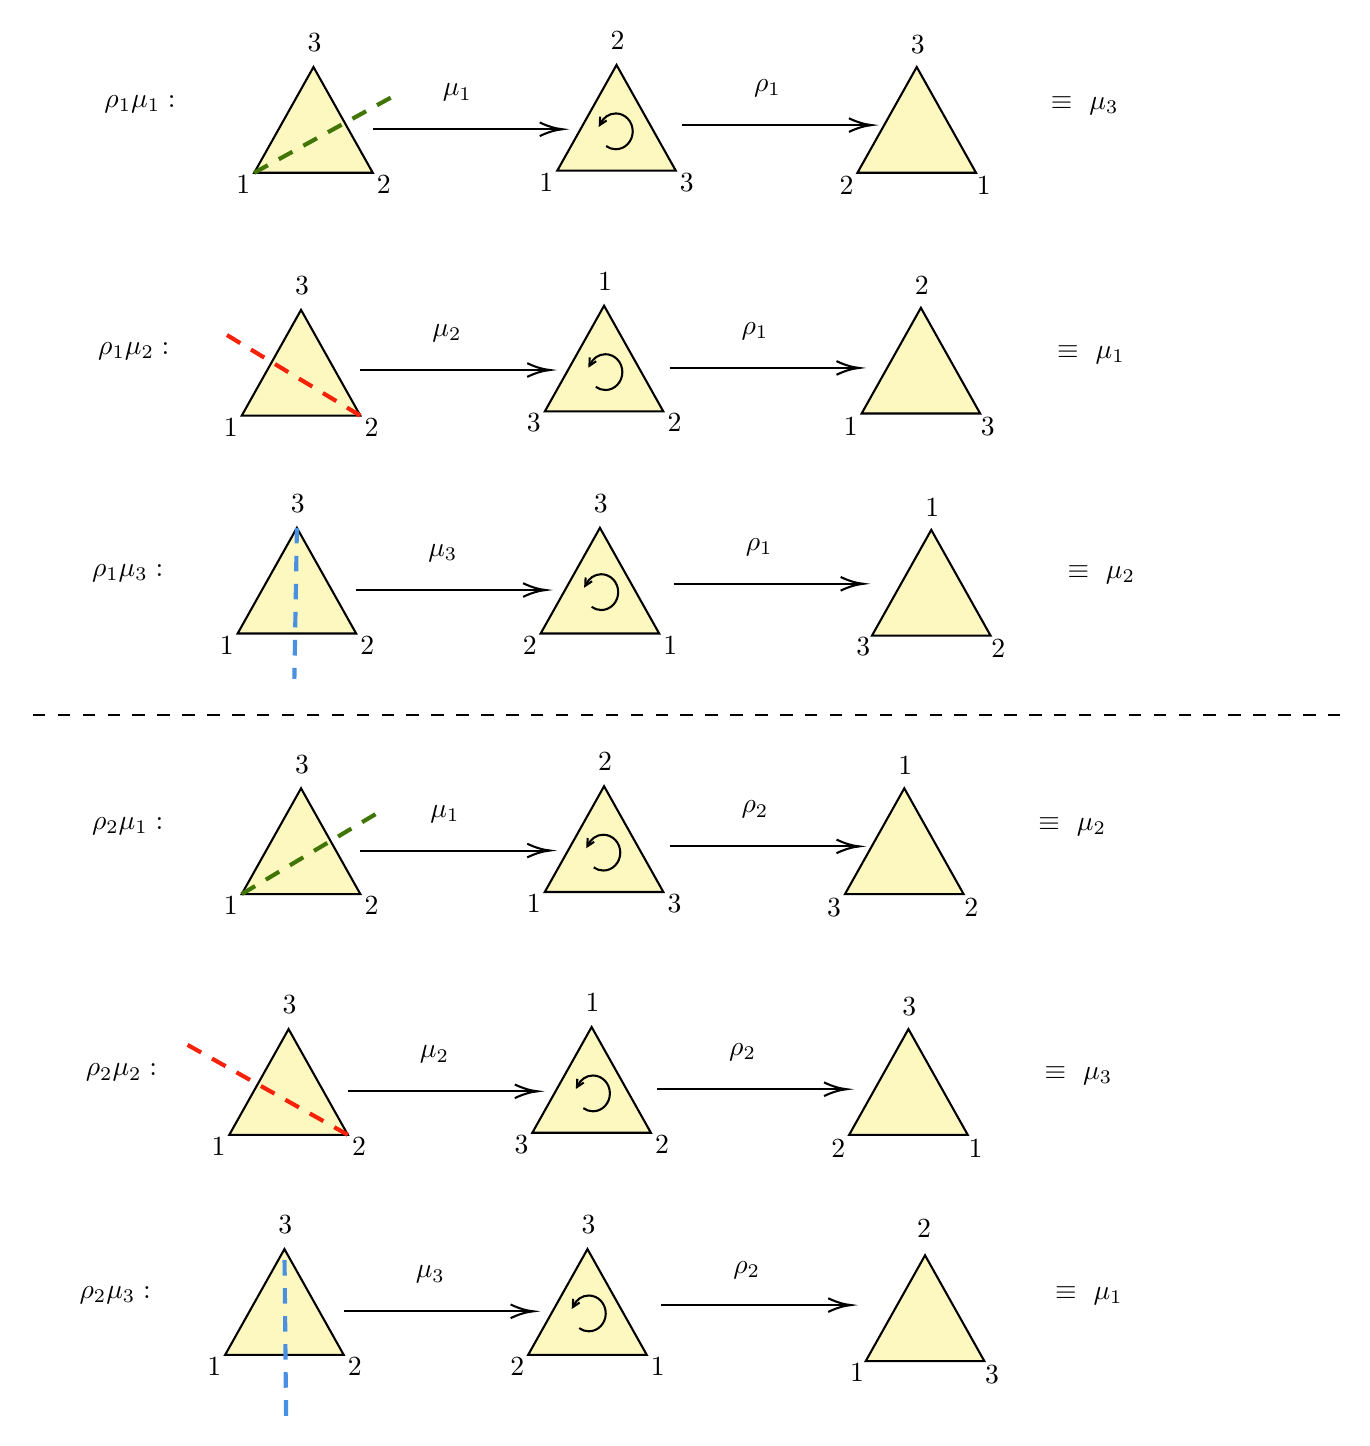
\begin{tikzpicture}[x=0.75pt,y=0.75pt,yscale=-1,xscale=1]
%uncomment if require: \path (0,848); %set diagram left start at 0, and has height of 848

%Shape: Triangle [id:dp19163829570612012] 
\draw  [fill={rgb, 255:red, 250; green, 238; blue, 106 }  ,fill opacity=0.43 ] (281.21,251.75) -- (309.76,302.69) -- (252.65,302.69) -- cycle ;

%Shape: Triangle [id:dp4514811151405802] 
\draw  [fill={rgb, 255:red, 250; green, 238; blue, 106 }  ,fill opacity=0.43 ] (283.21,144.75) -- (311.76,195.69) -- (254.65,195.69) -- cycle ;

%Shape: Triangle [id:dp2789857293750989] 
\draw  [fill={rgb, 255:red, 250; green, 238; blue, 106 }  ,fill opacity=0.43 ] (289.21,28.75) -- (317.76,79.69) -- (260.65,79.69) -- cycle ;

%Shape: Triangle [id:dp046781731174108665] 
\draw  [fill={rgb, 255:red, 250; green, 238; blue, 106 }  ,fill opacity=0.43 ] (435.85,145.75) -- (464.41,196.69) -- (407.29,196.69) -- cycle ;
%Shape: Triangle [id:dp21965592087989438] 
\draw  [fill={rgb, 255:red, 250; green, 238; blue, 106 }  ,fill opacity=0.43 ] (137.21,146.75) -- (165.76,197.69) -- (108.65,197.69) -- cycle ;

%Straight Lines [id:da6171044085428108] 
\draw    (314.75,174.73) -- (404.12,174.73) ;
\draw [shift={(406.12,174.73)}, rotate = 180] [color={rgb, 255:red, 0; green, 0; blue, 0 }  ][line width=0.75]    (10.93,-3.29) .. controls (6.95,-1.4) and (3.31,-0.3) .. (0,0) .. controls (3.31,0.3) and (6.95,1.4) .. (10.93,3.29)   ;
%Shape: Arc [id:dp18073662179695316] 
\draw  [draw opacity=0] (276.49,173.01) .. controls (277.81,170.11) and (280.61,168.11) .. (283.85,168.11) .. controls (288.36,168.11) and (292.01,171.97) .. (292.01,176.74) .. controls (292.01,181.5) and (288.36,185.37) .. (283.85,185.37) .. controls (282.13,185.37) and (280.53,184.8) .. (279.21,183.84) -- (283.85,176.74) -- cycle ; \draw   (276.49,173.01) .. controls (277.81,170.11) and (280.61,168.11) .. (283.85,168.11) .. controls (288.36,168.11) and (292.01,171.97) .. (292.01,176.74) .. controls (292.01,181.5) and (288.36,185.37) .. (283.85,185.37) .. controls (282.13,185.37) and (280.53,184.8) .. (279.21,183.84) ;  
\draw   (279.43,171.51) -- (276.15,173.67) -- (276.31,169.69) ;

%Straight Lines [id:da3068937473833855] 
\draw [color={rgb, 255:red, 247; green, 33; blue, 9 }  ,draw opacity=1 ][line width=1.5]  [dash pattern={on 5.63pt off 4.5pt}]  (165.76,197.69) -- (101,158.58) ;
%Straight Lines [id:da5998407578854817] 
\draw    (165.75,175.73) -- (255.12,175.73) ;
\draw [shift={(257.12,175.73)}, rotate = 180] [color={rgb, 255:red, 0; green, 0; blue, 0 }  ][line width=0.75]    (10.93,-3.29) .. controls (6.95,-1.4) and (3.31,-0.3) .. (0,0) .. controls (3.31,0.3) and (6.95,1.4) .. (10.93,3.29)   ;
%Shape: Triangle [id:dp6236283173447018] 
\draw  [fill={rgb, 255:red, 250; green, 238; blue, 106 }  ,fill opacity=0.43 ] (433.85,29.75) -- (462.41,80.69) -- (405.29,80.69) -- cycle ;
%Shape: Triangle [id:dp9148338393626184] 
\draw  [fill={rgb, 255:red, 250; green, 238; blue, 106 }  ,fill opacity=0.43 ] (143.21,29.75) -- (171.76,80.69) -- (114.65,80.69) -- cycle ;

%Straight Lines [id:da5291595834526982] 
\draw    (320.75,57.73) -- (410.12,57.73) ;
\draw [shift={(412.12,57.73)}, rotate = 180] [color={rgb, 255:red, 0; green, 0; blue, 0 }  ][line width=0.75]    (10.93,-3.29) .. controls (6.95,-1.4) and (3.31,-0.3) .. (0,0) .. controls (3.31,0.3) and (6.95,1.4) .. (10.93,3.29)   ;
%Shape: Arc [id:dp8806276716986381] 
\draw  [draw opacity=0] (281.49,57.01) .. controls (282.81,54.11) and (285.61,52.11) .. (288.85,52.11) .. controls (293.36,52.11) and (297.01,55.97) .. (297.01,60.74) .. controls (297.01,65.5) and (293.36,69.37) .. (288.85,69.37) .. controls (287.13,69.37) and (285.53,68.8) .. (284.21,67.84) -- (288.85,60.74) -- cycle ; \draw   (281.49,57.01) .. controls (282.81,54.11) and (285.61,52.11) .. (288.85,52.11) .. controls (293.36,52.11) and (297.01,55.97) .. (297.01,60.74) .. controls (297.01,65.5) and (293.36,69.37) .. (288.85,69.37) .. controls (287.13,69.37) and (285.53,68.8) .. (284.21,67.84) ;  
\draw   (284.43,55.51) -- (281.15,57.67) -- (281.31,53.69) ;

%Straight Lines [id:da1528001297367797] 
\draw    (171.75,59.73) -- (261.12,59.73) ;
\draw [shift={(263.12,59.73)}, rotate = 180] [color={rgb, 255:red, 0; green, 0; blue, 0 }  ][line width=0.75]    (10.93,-3.29) .. controls (6.95,-1.4) and (3.31,-0.3) .. (0,0) .. controls (3.31,0.3) and (6.95,1.4) .. (10.93,3.29)   ;
%Straight Lines [id:da9454860130046835] 
\draw [color={rgb, 255:red, 65; green, 117; blue, 5 }  ,draw opacity=1 ][line width=1.5]  [dash pattern={on 5.63pt off 4.5pt}]  (114.65,80.69) -- (181,44.2) ;
%Shape: Triangle [id:dp19435915537821324] 
\draw  [fill={rgb, 255:red, 250; green, 238; blue, 106 }  ,fill opacity=0.43 ] (440.85,252.75) -- (469.41,303.69) -- (412.29,303.69) -- cycle ;
%Shape: Triangle [id:dp018841163938158045] 
\draw  [fill={rgb, 255:red, 250; green, 238; blue, 106 }  ,fill opacity=0.43 ] (135.21,251.75) -- (163.76,302.69) -- (106.65,302.69) -- cycle ;

%Straight Lines [id:da43165367131576704] 
\draw    (316.75,278.73) -- (406.12,278.73) ;
\draw [shift={(408.12,278.73)}, rotate = 180] [color={rgb, 255:red, 0; green, 0; blue, 0 }  ][line width=0.75]    (10.93,-3.29) .. controls (6.95,-1.4) and (3.31,-0.3) .. (0,0) .. controls (3.31,0.3) and (6.95,1.4) .. (10.93,3.29)   ;
%Shape: Arc [id:dp469934169778089] 
\draw  [draw opacity=0] (274.49,279.01) .. controls (275.81,276.11) and (278.61,274.11) .. (281.85,274.11) .. controls (286.36,274.11) and (290.01,277.97) .. (290.01,282.74) .. controls (290.01,287.5) and (286.36,291.37) .. (281.85,291.37) .. controls (280.13,291.37) and (278.53,290.8) .. (277.21,289.84) -- (281.85,282.74) -- cycle ; \draw   (274.49,279.01) .. controls (275.81,276.11) and (278.61,274.11) .. (281.85,274.11) .. controls (286.36,274.11) and (290.01,277.97) .. (290.01,282.74) .. controls (290.01,287.5) and (286.36,291.37) .. (281.85,291.37) .. controls (280.13,291.37) and (278.53,290.8) .. (277.21,289.84) ;  
\draw   (277.43,277.51) -- (274.15,279.67) -- (274.31,275.69) ;

%Straight Lines [id:da8338747153912434] 
\draw    (163.75,281.73) -- (253.12,281.73) ;
\draw [shift={(255.12,281.73)}, rotate = 180] [color={rgb, 255:red, 0; green, 0; blue, 0 }  ][line width=0.75]    (10.93,-3.29) .. controls (6.95,-1.4) and (3.31,-0.3) .. (0,0) .. controls (3.31,0.3) and (6.95,1.4) .. (10.93,3.29)   ;
%Straight Lines [id:da4368451154360722] 
\draw [color={rgb, 255:red, 74; green, 144; blue, 226 }  ,draw opacity=1 ][line width=1.5]  [dash pattern={on 5.63pt off 4.5pt}]  (135.21,251.75) -- (134,324.58) ;
%Straight Lines [id:da39602756231413405] 
\draw  [dash pattern={on 4.5pt off 4.5pt}]  (638,341.9) -- (6,341.9) ;
%Shape: Triangle [id:dp6029455202280434] 
\draw  [fill={rgb, 255:red, 250; green, 238; blue, 106 }  ,fill opacity=0.43 ] (275.21,599.26) -- (303.76,650.2) -- (246.65,650.2) -- cycle ;

%Shape: Triangle [id:dp018595186853132772] 
\draw  [fill={rgb, 255:red, 250; green, 238; blue, 106 }  ,fill opacity=0.43 ] (277.21,492.26) -- (305.76,543.2) -- (248.65,543.2) -- cycle ;

%Shape: Triangle [id:dp1995520844656571] 
\draw  [fill={rgb, 255:red, 250; green, 238; blue, 106 }  ,fill opacity=0.43 ] (283.21,376.26) -- (311.76,427.2) -- (254.65,427.2) -- cycle ;

%Shape: Triangle [id:dp4516872025415908] 
\draw  [fill={rgb, 255:red, 250; green, 238; blue, 106 }  ,fill opacity=0.43 ] (429.85,493.26) -- (458.41,544.2) -- (401.29,544.2) -- cycle ;
%Shape: Triangle [id:dp016639459582723726] 
\draw  [fill={rgb, 255:red, 250; green, 238; blue, 106 }  ,fill opacity=0.43 ] (131.21,493.26) -- (159.76,544.2) -- (102.65,544.2) -- cycle ;

%Straight Lines [id:da2517410323346607] 
\draw    (308.75,522.24) -- (398.12,522.24) ;
\draw [shift={(400.12,522.24)}, rotate = 180] [color={rgb, 255:red, 0; green, 0; blue, 0 }  ][line width=0.75]    (10.93,-3.29) .. controls (6.95,-1.4) and (3.31,-0.3) .. (0,0) .. controls (3.31,0.3) and (6.95,1.4) .. (10.93,3.29)   ;
%Shape: Arc [id:dp5542020564776452] 
\draw  [draw opacity=0] (270.49,520.52) .. controls (271.81,517.63) and (274.61,515.62) .. (277.85,515.62) .. controls (282.36,515.62) and (286.01,519.49) .. (286.01,524.25) .. controls (286.01,529.02) and (282.36,532.88) .. (277.85,532.88) .. controls (276.13,532.88) and (274.53,532.31) .. (273.21,531.35) -- (277.85,524.25) -- cycle ; \draw   (270.49,520.52) .. controls (271.81,517.63) and (274.61,515.62) .. (277.85,515.62) .. controls (282.36,515.62) and (286.01,519.49) .. (286.01,524.25) .. controls (286.01,529.02) and (282.36,532.88) .. (277.85,532.88) .. controls (276.13,532.88) and (274.53,532.31) .. (273.21,531.35) ;  
\draw   (273.43,519.03) -- (270.15,521.18) -- (270.31,517.2) ;

%Straight Lines [id:da9302668125598431] 
\draw [color={rgb, 255:red, 247; green, 33; blue, 9 }  ,draw opacity=1 ][line width=1.5]  [dash pattern={on 5.63pt off 4.5pt}]  (159.76,544.2) -- (82,500.58) ;
%Straight Lines [id:da8637524871799385] 
\draw    (159.75,523.24) -- (249.12,523.24) ;
\draw [shift={(251.12,523.24)}, rotate = 180] [color={rgb, 255:red, 0; green, 0; blue, 0 }  ][line width=0.75]    (10.93,-3.29) .. controls (6.95,-1.4) and (3.31,-0.3) .. (0,0) .. controls (3.31,0.3) and (6.95,1.4) .. (10.93,3.29)   ;
%Shape: Triangle [id:dp5606675876112821] 
\draw  [fill={rgb, 255:red, 250; green, 238; blue, 106 }  ,fill opacity=0.43 ] (427.85,377.26) -- (456.41,428.2) -- (399.29,428.2) -- cycle ;
%Shape: Triangle [id:dp34393894000641356] 
\draw  [fill={rgb, 255:red, 250; green, 238; blue, 106 }  ,fill opacity=0.43 ] (137.21,377.26) -- (165.76,428.2) -- (108.65,428.2) -- cycle ;

%Straight Lines [id:da7822852564040057] 
\draw    (314.75,405.24) -- (404.12,405.24) ;
\draw [shift={(406.12,405.24)}, rotate = 180] [color={rgb, 255:red, 0; green, 0; blue, 0 }  ][line width=0.75]    (10.93,-3.29) .. controls (6.95,-1.4) and (3.31,-0.3) .. (0,0) .. controls (3.31,0.3) and (6.95,1.4) .. (10.93,3.29)   ;
%Shape: Arc [id:dp44211935360290144] 
\draw  [draw opacity=0] (275.49,404.52) .. controls (276.81,401.63) and (279.61,399.62) .. (282.85,399.62) .. controls (287.36,399.62) and (291.01,403.49) .. (291.01,408.25) .. controls (291.01,413.02) and (287.36,416.88) .. (282.85,416.88) .. controls (281.13,416.88) and (279.53,416.31) .. (278.21,415.35) -- (282.85,408.25) -- cycle ; \draw   (275.49,404.52) .. controls (276.81,401.63) and (279.61,399.62) .. (282.85,399.62) .. controls (287.36,399.62) and (291.01,403.49) .. (291.01,408.25) .. controls (291.01,413.02) and (287.36,416.88) .. (282.85,416.88) .. controls (281.13,416.88) and (279.53,416.31) .. (278.21,415.35) ;  
\draw   (278.43,403.03) -- (275.15,405.18) -- (275.31,401.2) ;

%Straight Lines [id:da0035615993293840464] 
\draw    (165.75,407.24) -- (255.12,407.24) ;
\draw [shift={(257.12,407.24)}, rotate = 180] [color={rgb, 255:red, 0; green, 0; blue, 0 }  ][line width=0.75]    (10.93,-3.29) .. controls (6.95,-1.4) and (3.31,-0.3) .. (0,0) .. controls (3.31,0.3) and (6.95,1.4) .. (10.93,3.29)   ;
%Straight Lines [id:da8500140614477428] 
\draw [color={rgb, 255:red, 65; green, 117; blue, 5 }  ,draw opacity=1 ][line width=1.5]  [dash pattern={on 5.63pt off 4.5pt}]  (108.65,428.2) -- (175,388.58) ;
%Shape: Triangle [id:dp705489061508623] 
\draw  [fill={rgb, 255:red, 250; green, 238; blue, 106 }  ,fill opacity=0.43 ] (437.85,602.26) -- (466.41,653.2) -- (409.29,653.2) -- cycle ;
%Shape: Triangle [id:dp20640781868355962] 
\draw  [fill={rgb, 255:red, 250; green, 238; blue, 106 }  ,fill opacity=0.43 ] (129.21,599.26) -- (157.76,650.2) -- (100.65,650.2) -- cycle ;

%Straight Lines [id:da275551010318138] 
\draw    (310.75,626.24) -- (400.12,626.24) ;
\draw [shift={(402.12,626.24)}, rotate = 180] [color={rgb, 255:red, 0; green, 0; blue, 0 }  ][line width=0.75]    (10.93,-3.29) .. controls (6.95,-1.4) and (3.31,-0.3) .. (0,0) .. controls (3.31,0.3) and (6.95,1.4) .. (10.93,3.29)   ;
%Shape: Arc [id:dp668827700841734] 
\draw  [draw opacity=0] (268.49,626.52) .. controls (269.81,623.63) and (272.61,621.62) .. (275.85,621.62) .. controls (280.36,621.62) and (284.01,625.49) .. (284.01,630.25) .. controls (284.01,635.02) and (280.36,638.88) .. (275.85,638.88) .. controls (274.13,638.88) and (272.53,638.31) .. (271.21,637.35) -- (275.85,630.25) -- cycle ; \draw   (268.49,626.52) .. controls (269.81,623.63) and (272.61,621.62) .. (275.85,621.62) .. controls (280.36,621.62) and (284.01,625.49) .. (284.01,630.25) .. controls (284.01,635.02) and (280.36,638.88) .. (275.85,638.88) .. controls (274.13,638.88) and (272.53,638.31) .. (271.21,637.35) ;  
\draw   (271.43,625.03) -- (268.15,627.18) -- (268.31,623.2) ;

%Straight Lines [id:da7833450093477451] 
\draw    (157.75,629.24) -- (247.12,629.24) ;
\draw [shift={(249.12,629.24)}, rotate = 180] [color={rgb, 255:red, 0; green, 0; blue, 0 }  ][line width=0.75]    (10.93,-3.29) .. controls (6.95,-1.4) and (3.31,-0.3) .. (0,0) .. controls (3.31,0.3) and (6.95,1.4) .. (10.93,3.29)   ;
%Straight Lines [id:da897202888338924] 
\draw [color={rgb, 255:red, 74; green, 144; blue, 226 }  ,draw opacity=1 ][line width=1.5]  [dash pattern={on 5.63pt off 4.5pt}]  (130,679.57) -- (129.21,599.26) ;

% Text Node
\draw (397.22,197.31) node [anchor=north west][inner sep=0.75pt]    {$1$};
% Text Node
\draw (463.3,197.31) node [anchor=north west][inner sep=0.75pt]    {$3$};
% Text Node
\draw (431.48,129.11) node [anchor=north west][inner sep=0.75pt]    {$2$};
% Text Node
\draw (348,151.4) node [anchor=north west][inner sep=0.75pt]    {$\rho _{1}$};
% Text Node
\draw (199,152.4) node [anchor=north west][inner sep=0.75pt]    {$\mu _{2}$};
% Text Node
\draw (505,268.4) node [anchor=north west][inner sep=0.75pt]    {$\equiv \ \mu _{2}$};
% Text Node
\draw (395.22,81.31) node [anchor=north west][inner sep=0.75pt]    {$2$};
% Text Node
\draw (461.3,81.31) node [anchor=north west][inner sep=0.75pt]    {$1$};
% Text Node
\draw (429.48,13.11) node [anchor=north west][inner sep=0.75pt]    {$3$};
% Text Node
\draw (354,34.4) node [anchor=north west][inner sep=0.75pt]    {$\rho _{1}$};
% Text Node
\draw (204,36.4) node [anchor=north west][inner sep=0.75pt]    {$\mu _{1}$};
% Text Node
\draw (500,162.4) node [anchor=north west][inner sep=0.75pt]    {$\equiv \ \mu _{1}$};
% Text Node
\draw (41,42.12) node [anchor=north west][inner sep=0.75pt]    {$\rho _{1} \mu _{1} :$};
% Text Node
\draw (38,161.12) node [anchor=north west][inner sep=0.75pt]    {$\rho _{1} \mu _{2} :$};
% Text Node
\draw (403.22,303.31) node [anchor=north west][inner sep=0.75pt]    {$3$};
% Text Node
\draw (468.3,304.31) node [anchor=north west][inner sep=0.75pt]    {$2$};
% Text Node
\draw (436.48,236.11) node [anchor=north west][inner sep=0.75pt]    {$1$};
% Text Node
\draw (350,255.4) node [anchor=north west][inner sep=0.75pt]    {$\rho _{1}$};
% Text Node
\draw (197,258.4) node [anchor=north west][inner sep=0.75pt]    {$\mu _{3}$};
% Text Node
\draw (497,42.4) node [anchor=north west][inner sep=0.75pt]    {$\equiv \ \mu _{3}$};
% Text Node
\draw (35,268.12) node [anchor=north west][inner sep=0.75pt]    {$\rho _{1} \mu _{3} :$};
% Text Node
\draw (276.84,234.29) node [anchor=north west][inner sep=0.75pt]    {$3$};
% Text Node
\draw (310.29,302.49) node [anchor=north west][inner sep=0.75pt]    {$1$};
% Text Node
\draw (242.57,302.49) node [anchor=north west][inner sep=0.75pt]    {$2$};
% Text Node
\draw (130.84,234.29) node [anchor=north west][inner sep=0.75pt]    {$3$};
% Text Node
\draw (164.29,302.49) node [anchor=north west][inner sep=0.75pt]    {$2$};
% Text Node
\draw (96.57,302.49) node [anchor=north west][inner sep=0.75pt]    {$1$};
% Text Node
\draw (284.84,11.29) node [anchor=north west][inner sep=0.75pt]    {$2$};
% Text Node
\draw (318.29,79.49) node [anchor=north west][inner sep=0.75pt]    {$3$};
% Text Node
\draw (250.57,79.49) node [anchor=north west][inner sep=0.75pt]    {$1$};
% Text Node
\draw (138.84,12.29) node [anchor=north west][inner sep=0.75pt]    {$3$};
% Text Node
\draw (172.29,80.49) node [anchor=north west][inner sep=0.75pt]    {$2$};
% Text Node
\draw (104.57,80.49) node [anchor=north west][inner sep=0.75pt]    {$1$};
% Text Node
\draw (278.84,127.29) node [anchor=north west][inner sep=0.75pt]    {$1$};
% Text Node
\draw (312.29,195.49) node [anchor=north west][inner sep=0.75pt]    {$2$};
% Text Node
\draw (244.57,195.49) node [anchor=north west][inner sep=0.75pt]    {$3$};
% Text Node
\draw (132.84,129.29) node [anchor=north west][inner sep=0.75pt]    {$3$};
% Text Node
\draw (166.29,197.49) node [anchor=north west][inner sep=0.75pt]    {$2$};
% Text Node
\draw (98.57,197.49) node [anchor=north west][inner sep=0.75pt]    {$1$};
% Text Node
\draw (391.22,544.82) node [anchor=north west][inner sep=0.75pt]    {$2$};
% Text Node
\draw (457.3,544.82) node [anchor=north west][inner sep=0.75pt]    {$1$};
% Text Node
\draw (425.48,476.62) node [anchor=north west][inner sep=0.75pt]    {$3$};
% Text Node
\draw (342,498.91) node [anchor=north west][inner sep=0.75pt]    {$\rho _{2}$};
% Text Node
\draw (193,499.91) node [anchor=north west][inner sep=0.75pt]    {$\mu _{2}$};
% Text Node
\draw (499,615.91) node [anchor=north west][inner sep=0.75pt]    {$\equiv \ \mu _{1}$};
% Text Node
\draw (389.22,428.82) node [anchor=north west][inner sep=0.75pt]    {$3$};
% Text Node
\draw (455.3,428.82) node [anchor=north west][inner sep=0.75pt]    {$2$};
% Text Node
\draw (423.48,360.62) node [anchor=north west][inner sep=0.75pt]    {$1$};
% Text Node
\draw (348,381.91) node [anchor=north west][inner sep=0.75pt]    {$\rho _{2}$};
% Text Node
\draw (198,383.91) node [anchor=north west][inner sep=0.75pt]    {$\mu _{1}$};
% Text Node
\draw (494,509.91) node [anchor=north west][inner sep=0.75pt]    {$\equiv \ \mu _{3}$};
% Text Node
\draw (35,389.63) node [anchor=north west][inner sep=0.75pt]    {$\rho _{2} \mu _{1} :$};
% Text Node
\draw (32,508.63) node [anchor=north west][inner sep=0.75pt]    {$\rho _{2} \mu _{2} :$};
% Text Node
\draw (400.22,652.82) node [anchor=north west][inner sep=0.75pt]    {$1$};
% Text Node
\draw (465.3,653.82) node [anchor=north west][inner sep=0.75pt]    {$3$};
% Text Node
\draw (432.48,583.62) node [anchor=north west][inner sep=0.75pt]    {$2$};
% Text Node
\draw (344,603.91) node [anchor=north west][inner sep=0.75pt]    {$\rho _{2}$};
% Text Node
\draw (191,605.91) node [anchor=north west][inner sep=0.75pt]    {$\mu _{3}$};
% Text Node
\draw (491,389.91) node [anchor=north west][inner sep=0.75pt]    {$\equiv \ \mu _{2}$};
% Text Node
\draw (29,615.63) node [anchor=north west][inner sep=0.75pt]    {$\rho _{2} \mu _{3} :$};
% Text Node
\draw (124.84,581.8) node [anchor=north west][inner sep=0.75pt]    {$3$};
% Text Node
\draw (158.29,650) node [anchor=north west][inner sep=0.75pt]    {$2$};
% Text Node
\draw (90.57,650) node [anchor=north west][inner sep=0.75pt]    {$1$};
% Text Node
\draw (132.84,359.8) node [anchor=north west][inner sep=0.75pt]    {$3$};
% Text Node
\draw (166.29,428) node [anchor=north west][inner sep=0.75pt]    {$2$};
% Text Node
\draw (98.57,428) node [anchor=north west][inner sep=0.75pt]    {$1$};
% Text Node
\draw (126.84,475.8) node [anchor=north west][inner sep=0.75pt]    {$3$};
% Text Node
\draw (160.29,544) node [anchor=north west][inner sep=0.75pt]    {$2$};
% Text Node
\draw (92.57,544) node [anchor=north west][inner sep=0.75pt]    {$1$};
% Text Node
\draw (278.84,358.8) node [anchor=north west][inner sep=0.75pt]    {$2$};
% Text Node
\draw (312.29,427) node [anchor=north west][inner sep=0.75pt]    {$3$};
% Text Node
\draw (244.57,427) node [anchor=north west][inner sep=0.75pt]    {$1$};
% Text Node
\draw (272.84,474.8) node [anchor=north west][inner sep=0.75pt]    {$1$};
% Text Node
\draw (306.29,543) node [anchor=north west][inner sep=0.75pt]    {$2$};
% Text Node
\draw (238.57,543) node [anchor=north west][inner sep=0.75pt]    {$3$};
% Text Node
\draw (270.84,581.8) node [anchor=north west][inner sep=0.75pt]    {$3$};
% Text Node
\draw (304.29,650) node [anchor=north west][inner sep=0.75pt]    {$1$};
% Text Node
\draw (236.57,650) node [anchor=north west][inner sep=0.75pt]    {$2$};


\end{tikzpicture}

\end{figure}
\begin{figure}[H]
    \centering
    

\tikzset{every picture/.style={line width=0.75pt}} %set default line width to 0.75pt        

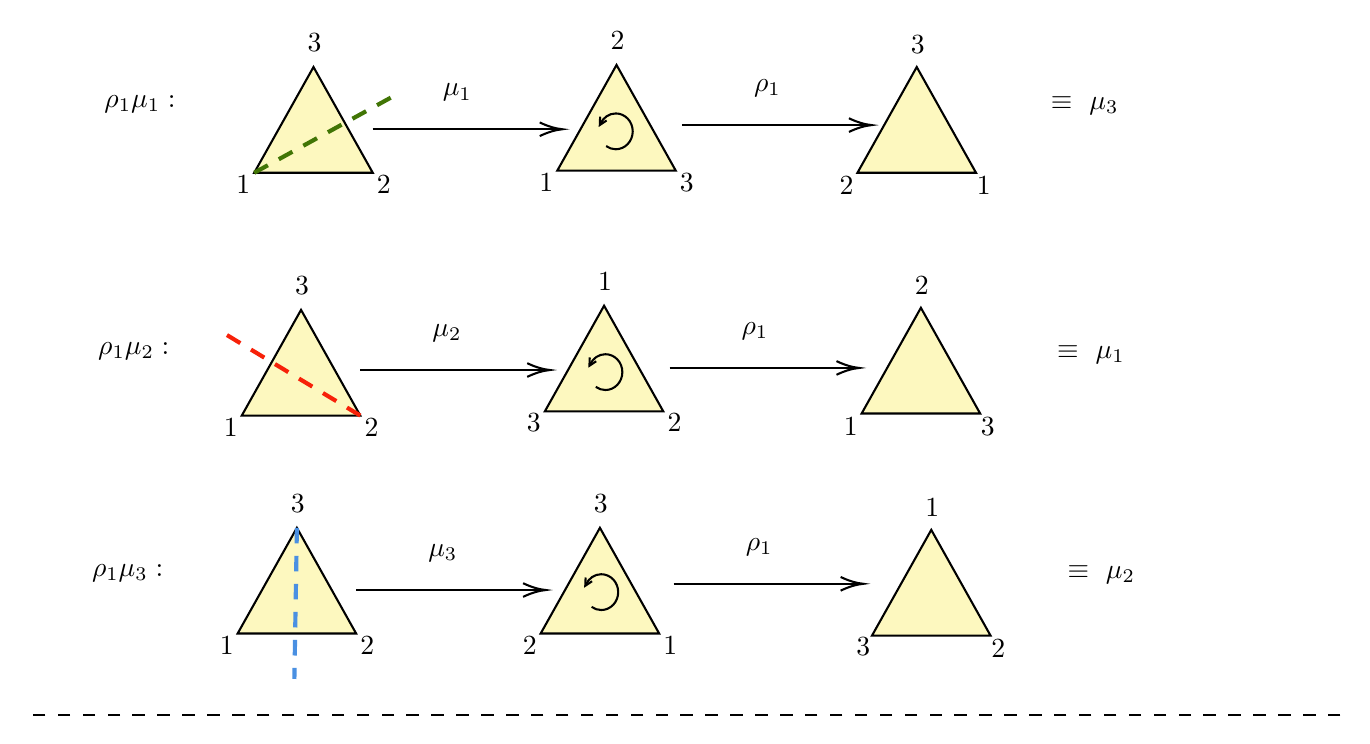
\begin{tikzpicture}[x=0.75pt,y=0.75pt,yscale=-1,xscale=1]
%uncomment if require: \path (0,350); %set diagram left start at 0, and has height of 350

%Shape: Triangle [id:dp19163829570612012] 
\draw  [fill={rgb, 255:red, 250; green, 238; blue, 106 }  ,fill opacity=0.43 ] (281.21,251.75) -- (309.76,302.69) -- (252.65,302.69) -- cycle ;

%Shape: Triangle [id:dp4514811151405802] 
\draw  [fill={rgb, 255:red, 250; green, 238; blue, 106 }  ,fill opacity=0.43 ] (283.21,144.75) -- (311.76,195.69) -- (254.65,195.69) -- cycle ;

%Shape: Triangle [id:dp2789857293750989] 
\draw  [fill={rgb, 255:red, 250; green, 238; blue, 106 }  ,fill opacity=0.43 ] (289.21,28.75) -- (317.76,79.69) -- (260.65,79.69) -- cycle ;

%Shape: Triangle [id:dp046781731174108665] 
\draw  [fill={rgb, 255:red, 250; green, 238; blue, 106 }  ,fill opacity=0.43 ] (435.85,145.75) -- (464.41,196.69) -- (407.29,196.69) -- cycle ;
%Shape: Triangle [id:dp21965592087989438] 
\draw  [fill={rgb, 255:red, 250; green, 238; blue, 106 }  ,fill opacity=0.43 ] (137.21,146.75) -- (165.76,197.69) -- (108.65,197.69) -- cycle ;

%Straight Lines [id:da6171044085428108] 
\draw    (314.75,174.73) -- (404.12,174.73) ;
\draw [shift={(406.12,174.73)}, rotate = 180] [color={rgb, 255:red, 0; green, 0; blue, 0 }  ][line width=0.75]    (10.93,-3.29) .. controls (6.95,-1.4) and (3.31,-0.3) .. (0,0) .. controls (3.31,0.3) and (6.95,1.4) .. (10.93,3.29)   ;
%Shape: Arc [id:dp18073662179695316] 
\draw  [draw opacity=0] (276.49,173.01) .. controls (277.81,170.11) and (280.61,168.11) .. (283.85,168.11) .. controls (288.36,168.11) and (292.01,171.97) .. (292.01,176.74) .. controls (292.01,181.5) and (288.36,185.37) .. (283.85,185.37) .. controls (282.13,185.37) and (280.53,184.8) .. (279.21,183.84) -- (283.85,176.74) -- cycle ; \draw   (276.49,173.01) .. controls (277.81,170.11) and (280.61,168.11) .. (283.85,168.11) .. controls (288.36,168.11) and (292.01,171.97) .. (292.01,176.74) .. controls (292.01,181.5) and (288.36,185.37) .. (283.85,185.37) .. controls (282.13,185.37) and (280.53,184.8) .. (279.21,183.84) ;  
\draw   (279.43,171.51) -- (276.15,173.67) -- (276.31,169.69) ;

%Straight Lines [id:da3068937473833855] 
\draw [color={rgb, 255:red, 247; green, 33; blue, 9 }  ,draw opacity=1 ][line width=1.5]  [dash pattern={on 5.63pt off 4.5pt}]  (165.76,197.69) -- (101,158.58) ;
%Straight Lines [id:da5998407578854817] 
\draw    (165.75,175.73) -- (255.12,175.73) ;
\draw [shift={(257.12,175.73)}, rotate = 180] [color={rgb, 255:red, 0; green, 0; blue, 0 }  ][line width=0.75]    (10.93,-3.29) .. controls (6.95,-1.4) and (3.31,-0.3) .. (0,0) .. controls (3.31,0.3) and (6.95,1.4) .. (10.93,3.29)   ;
%Shape: Triangle [id:dp6236283173447018] 
\draw  [fill={rgb, 255:red, 250; green, 238; blue, 106 }  ,fill opacity=0.43 ] (433.85,29.75) -- (462.41,80.69) -- (405.29,80.69) -- cycle ;
%Shape: Triangle [id:dp9148338393626184] 
\draw  [fill={rgb, 255:red, 250; green, 238; blue, 106 }  ,fill opacity=0.43 ] (143.21,29.75) -- (171.76,80.69) -- (114.65,80.69) -- cycle ;

%Straight Lines [id:da5291595834526982] 
\draw    (320.75,57.73) -- (410.12,57.73) ;
\draw [shift={(412.12,57.73)}, rotate = 180] [color={rgb, 255:red, 0; green, 0; blue, 0 }  ][line width=0.75]    (10.93,-3.29) .. controls (6.95,-1.4) and (3.31,-0.3) .. (0,0) .. controls (3.31,0.3) and (6.95,1.4) .. (10.93,3.29)   ;
%Shape: Arc [id:dp8806276716986381] 
\draw  [draw opacity=0] (281.49,57.01) .. controls (282.81,54.11) and (285.61,52.11) .. (288.85,52.11) .. controls (293.36,52.11) and (297.01,55.97) .. (297.01,60.74) .. controls (297.01,65.5) and (293.36,69.37) .. (288.85,69.37) .. controls (287.13,69.37) and (285.53,68.8) .. (284.21,67.84) -- (288.85,60.74) -- cycle ; \draw   (281.49,57.01) .. controls (282.81,54.11) and (285.61,52.11) .. (288.85,52.11) .. controls (293.36,52.11) and (297.01,55.97) .. (297.01,60.74) .. controls (297.01,65.5) and (293.36,69.37) .. (288.85,69.37) .. controls (287.13,69.37) and (285.53,68.8) .. (284.21,67.84) ;  
\draw   (284.43,55.51) -- (281.15,57.67) -- (281.31,53.69) ;

%Straight Lines [id:da1528001297367797] 
\draw    (171.75,59.73) -- (261.12,59.73) ;
\draw [shift={(263.12,59.73)}, rotate = 180] [color={rgb, 255:red, 0; green, 0; blue, 0 }  ][line width=0.75]    (10.93,-3.29) .. controls (6.95,-1.4) and (3.31,-0.3) .. (0,0) .. controls (3.31,0.3) and (6.95,1.4) .. (10.93,3.29)   ;
%Straight Lines [id:da9454860130046835] 
\draw [color={rgb, 255:red, 65; green, 117; blue, 5 }  ,draw opacity=1 ][line width=1.5]  [dash pattern={on 5.63pt off 4.5pt}]  (114.65,80.69) -- (181,44.2) ;
%Shape: Triangle [id:dp19435915537821324] 
\draw  [fill={rgb, 255:red, 250; green, 238; blue, 106 }  ,fill opacity=0.43 ] (440.85,252.75) -- (469.41,303.69) -- (412.29,303.69) -- cycle ;
%Shape: Triangle [id:dp018841163938158045] 
\draw  [fill={rgb, 255:red, 250; green, 238; blue, 106 }  ,fill opacity=0.43 ] (135.21,251.75) -- (163.76,302.69) -- (106.65,302.69) -- cycle ;

%Straight Lines [id:da43165367131576704] 
\draw    (316.75,278.73) -- (406.12,278.73) ;
\draw [shift={(408.12,278.73)}, rotate = 180] [color={rgb, 255:red, 0; green, 0; blue, 0 }  ][line width=0.75]    (10.93,-3.29) .. controls (6.95,-1.4) and (3.31,-0.3) .. (0,0) .. controls (3.31,0.3) and (6.95,1.4) .. (10.93,3.29)   ;
%Shape: Arc [id:dp469934169778089] 
\draw  [draw opacity=0] (274.49,279.01) .. controls (275.81,276.11) and (278.61,274.11) .. (281.85,274.11) .. controls (286.36,274.11) and (290.01,277.97) .. (290.01,282.74) .. controls (290.01,287.5) and (286.36,291.37) .. (281.85,291.37) .. controls (280.13,291.37) and (278.53,290.8) .. (277.21,289.84) -- (281.85,282.74) -- cycle ; \draw   (274.49,279.01) .. controls (275.81,276.11) and (278.61,274.11) .. (281.85,274.11) .. controls (286.36,274.11) and (290.01,277.97) .. (290.01,282.74) .. controls (290.01,287.5) and (286.36,291.37) .. (281.85,291.37) .. controls (280.13,291.37) and (278.53,290.8) .. (277.21,289.84) ;  
\draw   (277.43,277.51) -- (274.15,279.67) -- (274.31,275.69) ;

%Straight Lines [id:da8338747153912434] 
\draw    (163.75,281.73) -- (253.12,281.73) ;
\draw [shift={(255.12,281.73)}, rotate = 180] [color={rgb, 255:red, 0; green, 0; blue, 0 }  ][line width=0.75]    (10.93,-3.29) .. controls (6.95,-1.4) and (3.31,-0.3) .. (0,0) .. controls (3.31,0.3) and (6.95,1.4) .. (10.93,3.29)   ;
%Straight Lines [id:da4368451154360722] 
\draw [color={rgb, 255:red, 74; green, 144; blue, 226 }  ,draw opacity=1 ][line width=1.5]  [dash pattern={on 5.63pt off 4.5pt}]  (135.21,251.75) -- (134,324.58) ;
%Straight Lines [id:da39602756231413405] 
\draw  [dash pattern={on 4.5pt off 4.5pt}]  (638,341.9) -- (6,341.9) ;

% Text Node
\draw (397.22,197.31) node [anchor=north west][inner sep=0.75pt]    {$1$};
% Text Node
\draw (463.3,197.31) node [anchor=north west][inner sep=0.75pt]    {$3$};
% Text Node
\draw (431.48,129.11) node [anchor=north west][inner sep=0.75pt]    {$2$};
% Text Node
\draw (348,151.4) node [anchor=north west][inner sep=0.75pt]    {$\rho _{1}$};
% Text Node
\draw (199,152.4) node [anchor=north west][inner sep=0.75pt]    {$\mu _{2}$};
% Text Node
\draw (505,268.4) node [anchor=north west][inner sep=0.75pt]    {$\equiv \ \mu _{2}$};
% Text Node
\draw (395.22,81.31) node [anchor=north west][inner sep=0.75pt]    {$2$};
% Text Node
\draw (461.3,81.31) node [anchor=north west][inner sep=0.75pt]    {$1$};
% Text Node
\draw (429.48,13.11) node [anchor=north west][inner sep=0.75pt]    {$3$};
% Text Node
\draw (354,34.4) node [anchor=north west][inner sep=0.75pt]    {$\rho _{1}$};
% Text Node
\draw (204,36.4) node [anchor=north west][inner sep=0.75pt]    {$\mu _{1}$};
% Text Node
\draw (500,162.4) node [anchor=north west][inner sep=0.75pt]    {$\equiv \ \mu _{1}$};
% Text Node
\draw (41,42.12) node [anchor=north west][inner sep=0.75pt]    {$\rho _{1} \mu _{1} :$};
% Text Node
\draw (38,161.12) node [anchor=north west][inner sep=0.75pt]    {$\rho _{1} \mu _{2} :$};
% Text Node
\draw (403.22,303.31) node [anchor=north west][inner sep=0.75pt]    {$3$};
% Text Node
\draw (468.3,304.31) node [anchor=north west][inner sep=0.75pt]    {$2$};
% Text Node
\draw (436.48,236.11) node [anchor=north west][inner sep=0.75pt]    {$1$};
% Text Node
\draw (350,255.4) node [anchor=north west][inner sep=0.75pt]    {$\rho _{1}$};
% Text Node
\draw (197,258.4) node [anchor=north west][inner sep=0.75pt]    {$\mu _{3}$};
% Text Node
\draw (497,42.4) node [anchor=north west][inner sep=0.75pt]    {$\equiv \ \mu _{3}$};
% Text Node
\draw (35,268.12) node [anchor=north west][inner sep=0.75pt]    {$\rho _{1} \mu _{3} :$};
% Text Node
\draw (276.84,234.29) node [anchor=north west][inner sep=0.75pt]    {$3$};
% Text Node
\draw (310.29,302.49) node [anchor=north west][inner sep=0.75pt]    {$1$};
% Text Node
\draw (242.57,302.49) node [anchor=north west][inner sep=0.75pt]    {$2$};
% Text Node
\draw (130.84,234.29) node [anchor=north west][inner sep=0.75pt]    {$3$};
% Text Node
\draw (164.29,302.49) node [anchor=north west][inner sep=0.75pt]    {$2$};
% Text Node
\draw (96.57,302.49) node [anchor=north west][inner sep=0.75pt]    {$1$};
% Text Node
\draw (284.84,11.29) node [anchor=north west][inner sep=0.75pt]    {$2$};
% Text Node
\draw (318.29,79.49) node [anchor=north west][inner sep=0.75pt]    {$3$};
% Text Node
\draw (250.57,79.49) node [anchor=north west][inner sep=0.75pt]    {$1$};
% Text Node
\draw (138.84,12.29) node [anchor=north west][inner sep=0.75pt]    {$3$};
% Text Node
\draw (172.29,80.49) node [anchor=north west][inner sep=0.75pt]    {$2$};
% Text Node
\draw (104.57,80.49) node [anchor=north west][inner sep=0.75pt]    {$1$};
% Text Node
\draw (278.84,127.29) node [anchor=north west][inner sep=0.75pt]    {$1$};
% Text Node
\draw (312.29,195.49) node [anchor=north west][inner sep=0.75pt]    {$2$};
% Text Node
\draw (244.57,195.49) node [anchor=north west][inner sep=0.75pt]    {$3$};
% Text Node
\draw (132.84,129.29) node [anchor=north west][inner sep=0.75pt]    {$3$};
% Text Node
\draw (166.29,197.49) node [anchor=north west][inner sep=0.75pt]    {$2$};
% Text Node
\draw (98.57,197.49) node [anchor=north west][inner sep=0.75pt]    {$1$};


\end{tikzpicture}

\end{figure}
\begin{figure}[H]
    \centering
    

\tikzset{every picture/.style={line width=0.75pt}} %set default line width to 0.75pt        

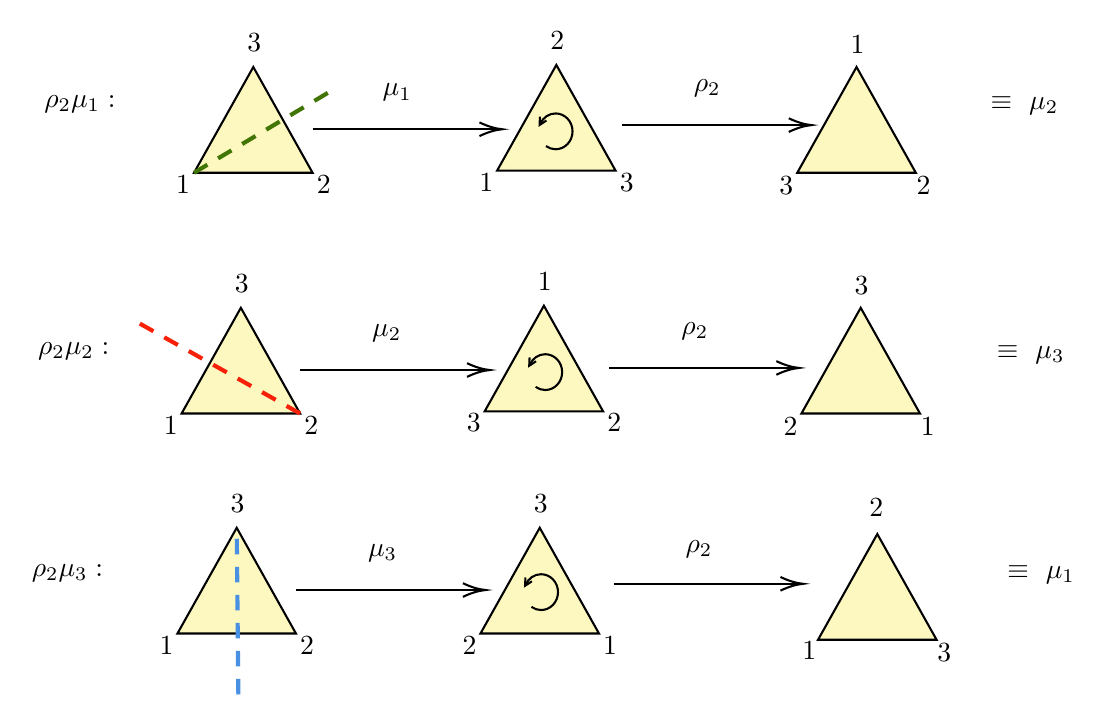
\begin{tikzpicture}[x=0.75pt,y=0.75pt,yscale=-1,xscale=1]
%uncomment if require: \path (0,341); %set diagram left start at 0, and has height of 341

%Shape: Triangle [id:dp38083149863639465] 
\draw  [fill={rgb, 255:red, 250; green, 238; blue, 106 }  ,fill opacity=0.43 ] (298.21,252.26) -- (326.76,303.2) -- (269.65,303.2) -- cycle ;

%Shape: Triangle [id:dp8834642070216787] 
\draw  [fill={rgb, 255:red, 250; green, 238; blue, 106 }  ,fill opacity=0.43 ] (300.21,145.26) -- (328.76,196.2) -- (271.65,196.2) -- cycle ;

%Shape: Triangle [id:dp8480067615213543] 
\draw  [fill={rgb, 255:red, 250; green, 238; blue, 106 }  ,fill opacity=0.43 ] (306.21,29.26) -- (334.76,80.2) -- (277.65,80.2) -- cycle ;

%Shape: Triangle [id:dp3963964289598798] 
\draw  [fill={rgb, 255:red, 250; green, 238; blue, 106 }  ,fill opacity=0.43 ] (452.85,146.26) -- (481.41,197.2) -- (424.29,197.2) -- cycle ;
%Shape: Triangle [id:dp7042235181906016] 
\draw  [fill={rgb, 255:red, 250; green, 238; blue, 106 }  ,fill opacity=0.43 ] (154.21,146.26) -- (182.76,197.2) -- (125.65,197.2) -- cycle ;

%Straight Lines [id:da513809238677429] 
\draw    (331.75,175.24) -- (421.12,175.24) ;
\draw [shift={(423.12,175.24)}, rotate = 180] [color={rgb, 255:red, 0; green, 0; blue, 0 }  ][line width=0.75]    (10.93,-3.29) .. controls (6.95,-1.4) and (3.31,-0.3) .. (0,0) .. controls (3.31,0.3) and (6.95,1.4) .. (10.93,3.29)   ;
%Shape: Arc [id:dp0752155899104685] 
\draw  [draw opacity=0] (293.49,173.52) .. controls (294.81,170.63) and (297.61,168.62) .. (300.85,168.62) .. controls (305.36,168.62) and (309.01,172.49) .. (309.01,177.25) .. controls (309.01,182.02) and (305.36,185.88) .. (300.85,185.88) .. controls (299.13,185.88) and (297.53,185.31) .. (296.21,184.35) -- (300.85,177.25) -- cycle ; \draw   (293.49,173.52) .. controls (294.81,170.63) and (297.61,168.62) .. (300.85,168.62) .. controls (305.36,168.62) and (309.01,172.49) .. (309.01,177.25) .. controls (309.01,182.02) and (305.36,185.88) .. (300.85,185.88) .. controls (299.13,185.88) and (297.53,185.31) .. (296.21,184.35) ;  
\draw   (296.43,172.03) -- (293.15,174.18) -- (293.31,170.2) ;

%Straight Lines [id:da014113470336568845] 
\draw [color={rgb, 255:red, 247; green, 33; blue, 9 }  ,draw opacity=1 ][line width=1.5]  [dash pattern={on 5.63pt off 4.5pt}]  (182.76,197.2) -- (105,153.58) ;
%Straight Lines [id:da4766267282251375] 
\draw    (182.75,176.24) -- (272.12,176.24) ;
\draw [shift={(274.12,176.24)}, rotate = 180] [color={rgb, 255:red, 0; green, 0; blue, 0 }  ][line width=0.75]    (10.93,-3.29) .. controls (6.95,-1.4) and (3.31,-0.3) .. (0,0) .. controls (3.31,0.3) and (6.95,1.4) .. (10.93,3.29)   ;
%Shape: Triangle [id:dp09853355186084745] 
\draw  [fill={rgb, 255:red, 250; green, 238; blue, 106 }  ,fill opacity=0.43 ] (450.85,30.26) -- (479.41,81.2) -- (422.29,81.2) -- cycle ;
%Shape: Triangle [id:dp024455387058983202] 
\draw  [fill={rgb, 255:red, 250; green, 238; blue, 106 }  ,fill opacity=0.43 ] (160.21,30.26) -- (188.76,81.2) -- (131.65,81.2) -- cycle ;

%Straight Lines [id:da4475565080931384] 
\draw    (337.75,58.24) -- (427.12,58.24) ;
\draw [shift={(429.12,58.24)}, rotate = 180] [color={rgb, 255:red, 0; green, 0; blue, 0 }  ][line width=0.75]    (10.93,-3.29) .. controls (6.95,-1.4) and (3.31,-0.3) .. (0,0) .. controls (3.31,0.3) and (6.95,1.4) .. (10.93,3.29)   ;
%Shape: Arc [id:dp7787418801052134] 
\draw  [draw opacity=0] (298.49,57.52) .. controls (299.81,54.63) and (302.61,52.62) .. (305.85,52.62) .. controls (310.36,52.62) and (314.01,56.49) .. (314.01,61.25) .. controls (314.01,66.02) and (310.36,69.88) .. (305.85,69.88) .. controls (304.13,69.88) and (302.53,69.31) .. (301.21,68.35) -- (305.85,61.25) -- cycle ; \draw   (298.49,57.52) .. controls (299.81,54.63) and (302.61,52.62) .. (305.85,52.62) .. controls (310.36,52.62) and (314.01,56.49) .. (314.01,61.25) .. controls (314.01,66.02) and (310.36,69.88) .. (305.85,69.88) .. controls (304.13,69.88) and (302.53,69.31) .. (301.21,68.35) ;  
\draw   (301.43,56.03) -- (298.15,58.18) -- (298.31,54.2) ;

%Straight Lines [id:da9005403767384724] 
\draw    (188.75,60.24) -- (278.12,60.24) ;
\draw [shift={(280.12,60.24)}, rotate = 180] [color={rgb, 255:red, 0; green, 0; blue, 0 }  ][line width=0.75]    (10.93,-3.29) .. controls (6.95,-1.4) and (3.31,-0.3) .. (0,0) .. controls (3.31,0.3) and (6.95,1.4) .. (10.93,3.29)   ;
%Straight Lines [id:da524115019147908] 
\draw [color={rgb, 255:red, 65; green, 117; blue, 5 }  ,draw opacity=1 ][line width=1.5]  [dash pattern={on 5.63pt off 4.5pt}]  (131.65,81.2) -- (198,41.58) ;
%Shape: Triangle [id:dp4811247244578286] 
\draw  [fill={rgb, 255:red, 250; green, 238; blue, 106 }  ,fill opacity=0.43 ] (460.85,255.26) -- (489.41,306.2) -- (432.29,306.2) -- cycle ;
%Shape: Triangle [id:dp23313243882490287] 
\draw  [fill={rgb, 255:red, 250; green, 238; blue, 106 }  ,fill opacity=0.43 ] (152.21,252.26) -- (180.76,303.2) -- (123.65,303.2) -- cycle ;

%Straight Lines [id:da1470468648823009] 
\draw    (333.75,279.24) -- (423.12,279.24) ;
\draw [shift={(425.12,279.24)}, rotate = 180] [color={rgb, 255:red, 0; green, 0; blue, 0 }  ][line width=0.75]    (10.93,-3.29) .. controls (6.95,-1.4) and (3.31,-0.3) .. (0,0) .. controls (3.31,0.3) and (6.95,1.4) .. (10.93,3.29)   ;
%Shape: Arc [id:dp34868135972523007] 
\draw  [draw opacity=0] (291.49,279.52) .. controls (292.81,276.63) and (295.61,274.62) .. (298.85,274.62) .. controls (303.36,274.62) and (307.01,278.49) .. (307.01,283.25) .. controls (307.01,288.02) and (303.36,291.88) .. (298.85,291.88) .. controls (297.13,291.88) and (295.53,291.31) .. (294.21,290.35) -- (298.85,283.25) -- cycle ; \draw   (291.49,279.52) .. controls (292.81,276.63) and (295.61,274.62) .. (298.85,274.62) .. controls (303.36,274.62) and (307.01,278.49) .. (307.01,283.25) .. controls (307.01,288.02) and (303.36,291.88) .. (298.85,291.88) .. controls (297.13,291.88) and (295.53,291.31) .. (294.21,290.35) ;  
\draw   (294.43,278.03) -- (291.15,280.18) -- (291.31,276.2) ;

%Straight Lines [id:da5341070876503803] 
\draw    (180.75,282.24) -- (270.12,282.24) ;
\draw [shift={(272.12,282.24)}, rotate = 180] [color={rgb, 255:red, 0; green, 0; blue, 0 }  ][line width=0.75]    (10.93,-3.29) .. controls (6.95,-1.4) and (3.31,-0.3) .. (0,0) .. controls (3.31,0.3) and (6.95,1.4) .. (10.93,3.29)   ;
%Straight Lines [id:da57458263235198] 
\draw [color={rgb, 255:red, 74; green, 144; blue, 226 }  ,draw opacity=1 ][line width=1.5]  [dash pattern={on 5.63pt off 4.5pt}]  (153,332.57) -- (152.21,252.26) ;

% Text Node
\draw (414.22,197.82) node [anchor=north west][inner sep=0.75pt]    {$2$};
% Text Node
\draw (480.3,197.82) node [anchor=north west][inner sep=0.75pt]    {$1$};
% Text Node
\draw (448.48,129.62) node [anchor=north west][inner sep=0.75pt]    {$3$};
% Text Node
\draw (365,151.91) node [anchor=north west][inner sep=0.75pt]    {$\rho _{2}$};
% Text Node
\draw (216,152.91) node [anchor=north west][inner sep=0.75pt]    {$\mu _{2}$};
% Text Node
\draw (522,268.91) node [anchor=north west][inner sep=0.75pt]    {$\equiv \ \mu _{1}$};
% Text Node
\draw (412.22,81.82) node [anchor=north west][inner sep=0.75pt]    {$3$};
% Text Node
\draw (478.3,81.82) node [anchor=north west][inner sep=0.75pt]    {$2$};
% Text Node
\draw (446.48,13.62) node [anchor=north west][inner sep=0.75pt]    {$1$};
% Text Node
\draw (371,34.91) node [anchor=north west][inner sep=0.75pt]    {$\rho _{2}$};
% Text Node
\draw (221,36.91) node [anchor=north west][inner sep=0.75pt]    {$\mu _{1}$};
% Text Node
\draw (517,162.91) node [anchor=north west][inner sep=0.75pt]    {$\equiv \ \mu _{3}$};
% Text Node
\draw (58,42.63) node [anchor=north west][inner sep=0.75pt]    {$\rho _{2} \mu _{1} :$};
% Text Node
\draw (55,161.63) node [anchor=north west][inner sep=0.75pt]    {$\rho _{2} \mu _{2} :$};
% Text Node
\draw (423.22,305.82) node [anchor=north west][inner sep=0.75pt]    {$1$};
% Text Node
\draw (488.3,306.82) node [anchor=north west][inner sep=0.75pt]    {$3$};
% Text Node
\draw (455.48,236.62) node [anchor=north west][inner sep=0.75pt]    {$2$};
% Text Node
\draw (367,256.91) node [anchor=north west][inner sep=0.75pt]    {$\rho _{2}$};
% Text Node
\draw (214,258.91) node [anchor=north west][inner sep=0.75pt]    {$\mu _{3}$};
% Text Node
\draw (514,42.91) node [anchor=north west][inner sep=0.75pt]    {$\equiv \ \mu _{2}$};
% Text Node
\draw (52,268.63) node [anchor=north west][inner sep=0.75pt]    {$\rho _{2} \mu _{3} :$};
% Text Node
\draw (147.84,234.8) node [anchor=north west][inner sep=0.75pt]    {$3$};
% Text Node
\draw (181.29,303) node [anchor=north west][inner sep=0.75pt]    {$2$};
% Text Node
\draw (113.57,303) node [anchor=north west][inner sep=0.75pt]    {$1$};
% Text Node
\draw (155.84,12.8) node [anchor=north west][inner sep=0.75pt]    {$3$};
% Text Node
\draw (189.29,81) node [anchor=north west][inner sep=0.75pt]    {$2$};
% Text Node
\draw (121.57,81) node [anchor=north west][inner sep=0.75pt]    {$1$};
% Text Node
\draw (149.84,128.8) node [anchor=north west][inner sep=0.75pt]    {$3$};
% Text Node
\draw (183.29,197) node [anchor=north west][inner sep=0.75pt]    {$2$};
% Text Node
\draw (115.57,197) node [anchor=north west][inner sep=0.75pt]    {$1$};
% Text Node
\draw (301.84,11.8) node [anchor=north west][inner sep=0.75pt]    {$2$};
% Text Node
\draw (335.29,80) node [anchor=north west][inner sep=0.75pt]    {$3$};
% Text Node
\draw (267.57,80) node [anchor=north west][inner sep=0.75pt]    {$1$};
% Text Node
\draw (295.84,127.8) node [anchor=north west][inner sep=0.75pt]    {$1$};
% Text Node
\draw (329.29,196) node [anchor=north west][inner sep=0.75pt]    {$2$};
% Text Node
\draw (261.57,196) node [anchor=north west][inner sep=0.75pt]    {$3$};
% Text Node
\draw (293.84,234.8) node [anchor=north west][inner sep=0.75pt]    {$3$};
% Text Node
\draw (327.29,303) node [anchor=north west][inner sep=0.75pt]    {$1$};
% Text Node
\draw (259.57,303) node [anchor=north west][inner sep=0.75pt]    {$2$};


\end{tikzpicture}

\end{figure}
\begin{figure}[H]
    \centering
    

\tikzset{every picture/.style={line width=0.75pt}} %set default line width to 0.75pt        

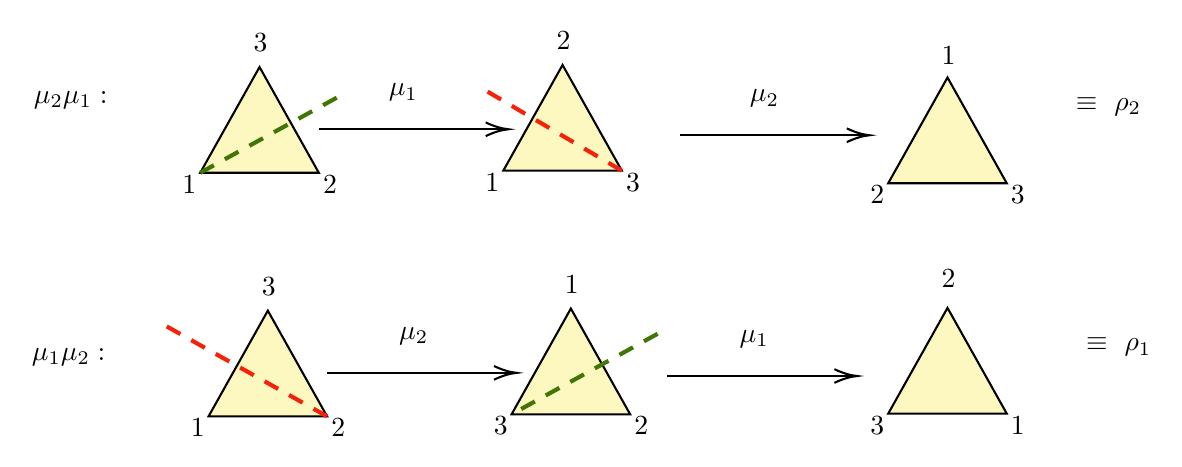
\begin{tikzpicture}[x=0.75pt,y=0.75pt,yscale=-1,xscale=1]
%uncomment if require: \path (0,227); %set diagram left start at 0, and has height of 227

%Straight Lines [id:da8577541306885849] 
\draw    (341.75,178.73) -- (431.12,178.73) ;
\draw [shift={(433.12,178.73)}, rotate = 180] [color={rgb, 255:red, 0; green, 0; blue, 0 }  ][line width=0.75]    (10.93,-3.29) .. controls (6.95,-1.4) and (3.31,-0.3) .. (0,0) .. controls (3.31,0.3) and (6.95,1.4) .. (10.93,3.29)   ;
%Straight Lines [id:da14363701357932668] 
\draw    (347.75,62.73) -- (437.12,62.73) ;
\draw [shift={(439.12,62.73)}, rotate = 180] [color={rgb, 255:red, 0; green, 0; blue, 0 }  ][line width=0.75]    (10.93,-3.29) .. controls (6.95,-1.4) and (3.31,-0.3) .. (0,0) .. controls (3.31,0.3) and (6.95,1.4) .. (10.93,3.29)   ;
%Shape: Triangle [id:dp6166967616717672] 
\draw  [fill={rgb, 255:red, 250; green, 238; blue, 106 }  ,fill opacity=0.43 ] (476.67,34.9) -- (505.22,85.84) -- (448.11,85.84) -- cycle ;
%Shape: Triangle [id:dp10184292255708727] 
\draw  [fill={rgb, 255:red, 250; green, 238; blue, 106 }  ,fill opacity=0.43 ] (476.67,145.9) -- (505.22,196.84) -- (448.11,196.84) -- cycle ;
%Shape: Triangle [id:dp16072718880753045] 
\draw  [fill={rgb, 255:red, 250; green, 238; blue, 106 }  ,fill opacity=0.43 ] (291.21,28.86) -- (319.76,79.8) -- (262.65,79.8) -- cycle ;

%Shape: Triangle [id:dp5648577801345768] 
\draw  [fill={rgb, 255:red, 250; green, 238; blue, 106 }  ,fill opacity=0.43 ] (145.21,29.86) -- (173.76,80.8) -- (116.65,80.8) -- cycle ;

%Straight Lines [id:da2701519616679303] 
\draw    (173.75,59.84) -- (263.12,59.84) ;
\draw [shift={(265.12,59.84)}, rotate = 180] [color={rgb, 255:red, 0; green, 0; blue, 0 }  ][line width=0.75]    (10.93,-3.29) .. controls (6.95,-1.4) and (3.31,-0.3) .. (0,0) .. controls (3.31,0.3) and (6.95,1.4) .. (10.93,3.29)   ;
%Straight Lines [id:da8423035151742334] 
\draw [color={rgb, 255:red, 65; green, 117; blue, 5 }  ,draw opacity=1 ][line width=1.5]  [dash pattern={on 5.63pt off 4.5pt}]  (116.65,80.8) -- (183,44.31) ;
%Shape: Triangle [id:dp6294228660813018] 
\draw  [fill={rgb, 255:red, 250; green, 238; blue, 106 }  ,fill opacity=0.43 ] (295.21,146.23) -- (323.76,197.17) -- (266.65,197.17) -- cycle ;

%Shape: Triangle [id:dp25618566511022456] 
\draw  [fill={rgb, 255:red, 250; green, 238; blue, 106 }  ,fill opacity=0.43 ] (149.21,147.23) -- (177.76,198.17) -- (120.65,198.17) -- cycle ;

%Straight Lines [id:da8827959373008387] 
\draw [color={rgb, 255:red, 247; green, 33; blue, 9 }  ,draw opacity=1 ][line width=1.5]  [dash pattern={on 5.63pt off 4.5pt}]  (177.76,198.17) -- (100,154.55) ;
%Straight Lines [id:da40930653904783754] 
\draw    (177.75,177.21) -- (267.12,177.21) ;
\draw [shift={(269.12,177.21)}, rotate = 180] [color={rgb, 255:red, 0; green, 0; blue, 0 }  ][line width=0.75]    (10.93,-3.29) .. controls (6.95,-1.4) and (3.31,-0.3) .. (0,0) .. controls (3.31,0.3) and (6.95,1.4) .. (10.93,3.29)   ;
%Straight Lines [id:da4786144067411211] 
\draw [color={rgb, 255:red, 247; green, 33; blue, 9 }  ,draw opacity=1 ][line width=1.5]  [dash pattern={on 5.63pt off 4.5pt}]  (319.76,79.8) -- (252,39.9) ;
%Straight Lines [id:da1460315703759597] 
\draw [color={rgb, 255:red, 65; green, 117; blue, 5 }  ,draw opacity=1 ][line width=1.5]  [dash pattern={on 5.63pt off 4.5pt}]  (337,158.38) -- (266.65,197.17) ;

% Text Node
\draw (34,164.12) node [anchor=north west][inner sep=0.75pt]    {$\mu _{1} \mu _{2} :$};
% Text Node
\draw (35,40.12) node [anchor=north west][inner sep=0.75pt]    {$\mu _{2} \mu _{1} :$};
% Text Node
\draw (375,155.4) node [anchor=north west][inner sep=0.75pt]    {$\mu _{1}$};
% Text Node
\draw (380,39.4) node [anchor=north west][inner sep=0.75pt]    {$\mu _{2}$};
% Text Node
\draw (438.03,85.64) node [anchor=north west][inner sep=0.75pt]    {$2$};
% Text Node
\draw (505.75,85.64) node [anchor=north west][inner sep=0.75pt]    {$3$};
% Text Node
\draw (472.3,18.44) node [anchor=north west][inner sep=0.75pt]    {$1$};
% Text Node
\draw (438.03,196.64) node [anchor=north west][inner sep=0.75pt]    {$3$};
% Text Node
\draw (505.75,196.64) node [anchor=north west][inner sep=0.75pt]    {$1$};
% Text Node
\draw (472.3,125.92) node [anchor=north west][inner sep=0.75pt]    {$2$};
% Text Node
\draw (206,36.51) node [anchor=north west][inner sep=0.75pt]    {$\mu _{1}$};
% Text Node
\draw (211,153.88) node [anchor=north west][inner sep=0.75pt]    {$\mu _{2}$};
% Text Node
\draw (537,42.97) node [anchor=north west][inner sep=0.75pt]    {$\equiv \ \rho _{2}$};
% Text Node
\draw (542,158.97) node [anchor=north west][inner sep=0.75pt]    {$\equiv \ \rho _{1}$};
% Text Node
\draw (144.84,129.77) node [anchor=north west][inner sep=0.75pt]    {$3$};
% Text Node
\draw (178.29,197.97) node [anchor=north west][inner sep=0.75pt]    {$2$};
% Text Node
\draw (110.57,197.97) node [anchor=north west][inner sep=0.75pt]    {$1$};
% Text Node
\draw (290.84,128.77) node [anchor=north west][inner sep=0.75pt]    {$1$};
% Text Node
\draw (324.29,196.97) node [anchor=north west][inner sep=0.75pt]    {$2$};
% Text Node
\draw (256.57,196.97) node [anchor=north west][inner sep=0.75pt]    {$3$};
% Text Node
\draw (140.84,12.4) node [anchor=north west][inner sep=0.75pt]    {$3$};
% Text Node
\draw (174.29,80.6) node [anchor=north west][inner sep=0.75pt]    {$2$};
% Text Node
\draw (106.57,80.6) node [anchor=north west][inner sep=0.75pt]    {$1$};
% Text Node
\draw (286.84,11.4) node [anchor=north west][inner sep=0.75pt]    {$2$};
% Text Node
\draw (320.29,79.6) node [anchor=north west][inner sep=0.75pt]    {$3$};
% Text Node
\draw (252.57,79.6) node [anchor=north west][inner sep=0.75pt]    {$1$};


\end{tikzpicture}

\end{figure}
\begin{figure}[H]
    \centering
    

\tikzset{every picture/.style={line width=0.75pt}} %set default line width to 0.75pt        

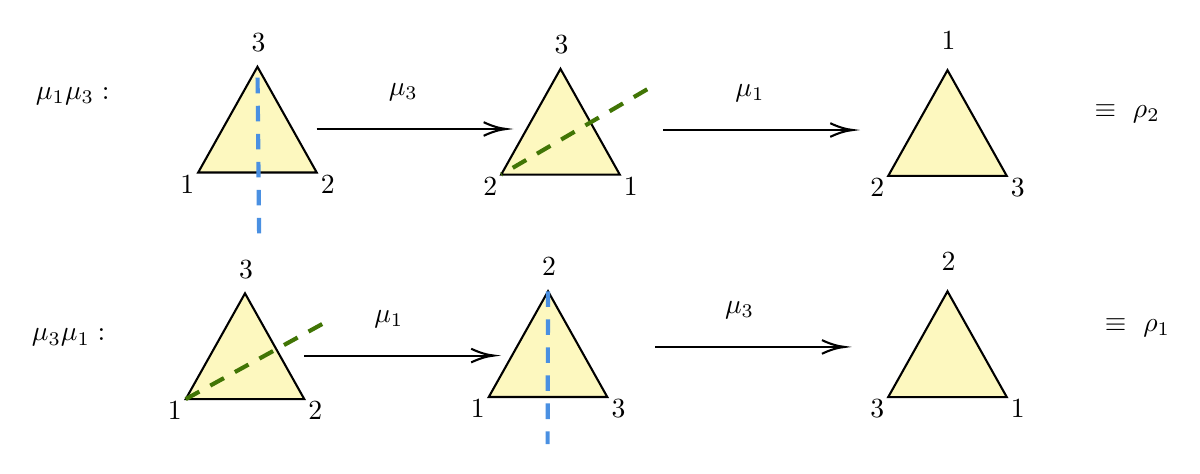
\begin{tikzpicture}[x=0.75pt,y=0.75pt,yscale=-1,xscale=1]
%uncomment if require: \path (0,213); %set diagram left start at 0, and has height of 213

%Straight Lines [id:da23227613985646378] 
\draw    (346.75,55.73) -- (436.12,55.73) ;
\draw [shift={(438.12,55.73)}, rotate = 180] [color={rgb, 255:red, 0; green, 0; blue, 0 }  ][line width=0.75]    (10.93,-3.29) .. controls (6.95,-1.4) and (3.31,-0.3) .. (0,0) .. controls (3.31,0.3) and (6.95,1.4) .. (10.93,3.29)   ;
%Straight Lines [id:da2537972233308252] 
\draw    (342.75,160.24) -- (432.12,160.24) ;
\draw [shift={(434.12,160.24)}, rotate = 180] [color={rgb, 255:red, 0; green, 0; blue, 0 }  ][line width=0.75]    (10.93,-3.29) .. controls (6.95,-1.4) and (3.31,-0.3) .. (0,0) .. controls (3.31,0.3) and (6.95,1.4) .. (10.93,3.29)   ;
%Shape: Triangle [id:dp5138384240785593] 
\draw  [fill={rgb, 255:red, 250; green, 238; blue, 106 }  ,fill opacity=0.43 ] (483.67,26.9) -- (512.22,77.84) -- (455.11,77.84) -- cycle ;
%Shape: Triangle [id:dp9299490724469842] 
\draw  [fill={rgb, 255:red, 250; green, 238; blue, 106 }  ,fill opacity=0.43 ] (483.67,133.45) -- (512.22,184.39) -- (455.11,184.39) -- cycle ;
%Shape: Triangle [id:dp3094198210232113] 
\draw  [fill={rgb, 255:red, 250; green, 238; blue, 106 }  ,fill opacity=0.43 ] (291.21,133.43) -- (319.76,184.37) -- (262.65,184.37) -- cycle ;

%Shape: Triangle [id:dp6072285341774635] 
\draw  [fill={rgb, 255:red, 250; green, 238; blue, 106 }  ,fill opacity=0.43 ] (145.21,134.43) -- (173.76,185.37) -- (116.65,185.37) -- cycle ;

%Straight Lines [id:da9916566252372986] 
\draw    (173.75,164.4) -- (263.12,164.4) ;
\draw [shift={(265.12,164.4)}, rotate = 180] [color={rgb, 255:red, 0; green, 0; blue, 0 }  ][line width=0.75]    (10.93,-3.29) .. controls (6.95,-1.4) and (3.31,-0.3) .. (0,0) .. controls (3.31,0.3) and (6.95,1.4) .. (10.93,3.29)   ;
%Straight Lines [id:da3884795444667827] 
\draw [color={rgb, 255:red, 65; green, 117; blue, 5 }  ,draw opacity=1 ][line width=1.5]  [dash pattern={on 5.63pt off 4.5pt}]  (116.65,185.37) -- (183,148.88) ;
%Shape: Triangle [id:dp4067226035070607] 
\draw  [fill={rgb, 255:red, 250; green, 238; blue, 106 }  ,fill opacity=0.43 ] (297.21,26.26) -- (325.76,77.2) -- (268.65,77.2) -- cycle ;

%Shape: Triangle [id:dp737332924910008] 
\draw  [fill={rgb, 255:red, 250; green, 238; blue, 106 }  ,fill opacity=0.43 ] (151.21,25.26) -- (179.76,76.2) -- (122.65,76.2) -- cycle ;

%Straight Lines [id:da7337740639590441] 
\draw    (179.75,55.24) -- (269.12,55.24) ;
\draw [shift={(271.12,55.24)}, rotate = 180] [color={rgb, 255:red, 0; green, 0; blue, 0 }  ][line width=0.75]    (10.93,-3.29) .. controls (6.95,-1.4) and (3.31,-0.3) .. (0,0) .. controls (3.31,0.3) and (6.95,1.4) .. (10.93,3.29)   ;
%Straight Lines [id:da9237438755224345] 
\draw [color={rgb, 255:red, 74; green, 144; blue, 226 }  ,draw opacity=1 ][line width=1.5]  [dash pattern={on 5.63pt off 4.5pt}]  (152,105.57) -- (151.21,25.26) ;
%Straight Lines [id:da1778028966163362] 
\draw [color={rgb, 255:red, 74; green, 144; blue, 226 }  ,draw opacity=1 ][line width=1.5]  [dash pattern={on 5.63pt off 4.5pt}]  (291.21,133.43) -- (291,207.1) ;
%Straight Lines [id:da5297072499212381] 
\draw [color={rgb, 255:red, 65; green, 117; blue, 5 }  ,draw opacity=1 ][line width=1.5]  [dash pattern={on 5.63pt off 4.5pt}]  (339,36.1) -- (268.65,77.2) ;

% Text Node
\draw (41,150.12) node [anchor=north west][inner sep=0.75pt]    {$\mu _{3} \mu _{1} :$};
% Text Node
\draw (43,33.63) node [anchor=north west][inner sep=0.75pt]    {$\mu _{1} \mu _{3} :$};
% Text Node
\draw (380,32.4) node [anchor=north west][inner sep=0.75pt]    {$\mu _{1}$};
% Text Node
\draw (375,136.91) node [anchor=north west][inner sep=0.75pt]    {$\mu _{3}$};
% Text Node
\draw (445.03,77.64) node [anchor=north west][inner sep=0.75pt]    {$2$};
% Text Node
\draw (512.75,77.64) node [anchor=north west][inner sep=0.75pt]    {$3$};
% Text Node
\draw (479.3,6.92) node [anchor=north west][inner sep=0.75pt]    {$1$};
% Text Node
\draw (445.03,184.19) node [anchor=north west][inner sep=0.75pt]    {$3$};
% Text Node
\draw (512.75,184.19) node [anchor=north west][inner sep=0.75pt]    {$1$};
% Text Node
\draw (479.3,113.47) node [anchor=north west][inner sep=0.75pt]    {$2$};
% Text Node
\draw (206,141.08) node [anchor=north west][inner sep=0.75pt]    {$\mu _{1}$};
% Text Node
\draw (213,31.91) node [anchor=north west][inner sep=0.75pt]    {$\mu _{3}$};
% Text Node
\draw (553,41.97) node [anchor=north west][inner sep=0.75pt]    {$\equiv \ \rho _{2}$};
% Text Node
\draw (558,144.97) node [anchor=north west][inner sep=0.75pt]    {$\equiv \ \rho _{1}$};
% Text Node
\draw (146.84,7.8) node [anchor=north west][inner sep=0.75pt]    {$3$};
% Text Node
\draw (180.29,76) node [anchor=north west][inner sep=0.75pt]    {$2$};
% Text Node
\draw (112.57,76) node [anchor=north west][inner sep=0.75pt]    {$1$};
% Text Node
\draw (292.84,8.8) node [anchor=north west][inner sep=0.75pt]    {$3$};
% Text Node
\draw (326.29,77) node [anchor=north west][inner sep=0.75pt]    {$1$};
% Text Node
\draw (258.57,77) node [anchor=north west][inner sep=0.75pt]    {$2$};
% Text Node
\draw (140.84,116.97) node [anchor=north west][inner sep=0.75pt]    {$3$};
% Text Node
\draw (174.29,185.17) node [anchor=north west][inner sep=0.75pt]    {$2$};
% Text Node
\draw (106.57,185.17) node [anchor=north west][inner sep=0.75pt]    {$1$};
% Text Node
\draw (286.84,115.97) node [anchor=north west][inner sep=0.75pt]    {$2$};
% Text Node
\draw (320.29,184.17) node [anchor=north west][inner sep=0.75pt]    {$3$};
% Text Node
\draw (252.57,184.17) node [anchor=north west][inner sep=0.75pt]    {$1$};


\end{tikzpicture}

\end{figure}
\begin{figure}[H]
    \centering
    

\tikzset{every picture/.style={line width=0.75pt}} %set default line width to 0.75pt        

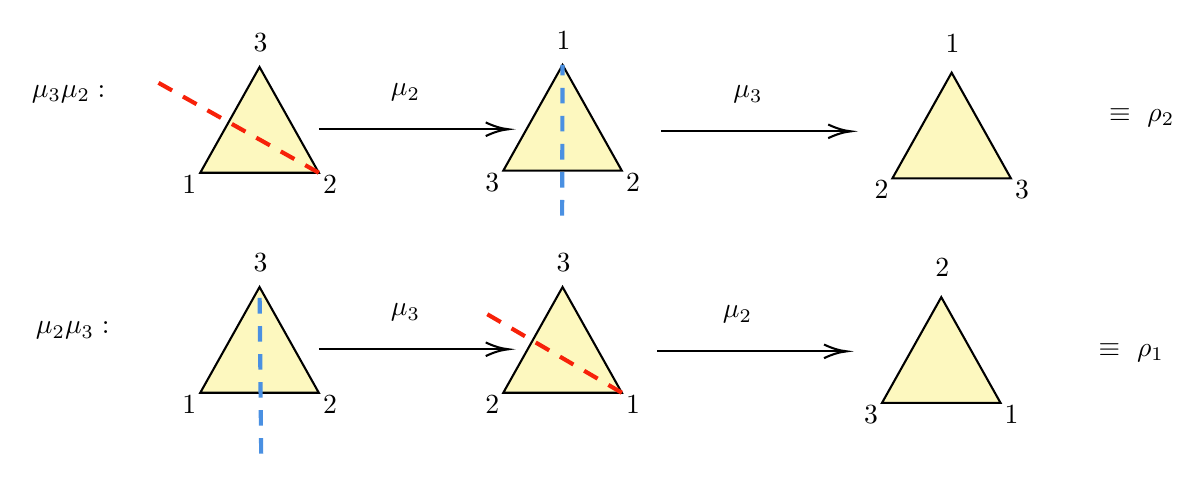
\begin{tikzpicture}[x=0.75pt,y=0.75pt,yscale=-1,xscale=1]
%uncomment if require: \path (0,222); %set diagram left start at 0, and has height of 222

%Straight Lines [id:da07468523150361062] 
\draw    (365.75,63.24) -- (455.12,63.24) ;
\draw [shift={(457.12,63.24)}, rotate = 180] [color={rgb, 255:red, 0; green, 0; blue, 0 }  ][line width=0.75]    (10.93,-3.29) .. controls (6.95,-1.4) and (3.31,-0.3) .. (0,0) .. controls (3.31,0.3) and (6.95,1.4) .. (10.93,3.29)   ;
%Straight Lines [id:da7303972534757194] 
\draw    (363.75,169.24) -- (453.12,169.24) ;
\draw [shift={(455.12,169.24)}, rotate = 180] [color={rgb, 255:red, 0; green, 0; blue, 0 }  ][line width=0.75]    (10.93,-3.29) .. controls (6.95,-1.4) and (3.31,-0.3) .. (0,0) .. controls (3.31,0.3) and (6.95,1.4) .. (10.93,3.29)   ;
%Shape: Triangle [id:dp3013799303944148] 
\draw  [fill={rgb, 255:red, 250; green, 238; blue, 106 }  ,fill opacity=0.43 ] (505.67,34.97) -- (534.22,85.91) -- (477.11,85.91) -- cycle ;
%Shape: Triangle [id:dp8366420155668731] 
\draw  [fill={rgb, 255:red, 250; green, 238; blue, 106 }  ,fill opacity=0.43 ] (500.67,143.13) -- (529.22,194.08) -- (472.11,194.08) -- cycle ;
%Shape: Triangle [id:dp08911820327135123] 
\draw  [fill={rgb, 255:red, 250; green, 238; blue, 106 }  ,fill opacity=0.43 ] (318.21,31.26) -- (346.76,82.2) -- (289.65,82.2) -- cycle ;

%Shape: Triangle [id:dp6959388954166472] 
\draw  [fill={rgb, 255:red, 250; green, 238; blue, 106 }  ,fill opacity=0.43 ] (172.21,32.26) -- (200.76,83.2) -- (143.65,83.2) -- cycle ;

%Straight Lines [id:da28918778113624566] 
\draw [color={rgb, 255:red, 247; green, 33; blue, 9 }  ,draw opacity=1 ][line width=1.5]  [dash pattern={on 5.63pt off 4.5pt}]  (200.76,83.2) -- (123,39.58) ;
%Straight Lines [id:da8925263126633919] 
\draw    (200.75,62.24) -- (290.12,62.24) ;
\draw [shift={(292.12,62.24)}, rotate = 180] [color={rgb, 255:red, 0; green, 0; blue, 0 }  ][line width=0.75]    (10.93,-3.29) .. controls (6.95,-1.4) and (3.31,-0.3) .. (0,0) .. controls (3.31,0.3) and (6.95,1.4) .. (10.93,3.29)   ;
%Shape: Triangle [id:dp5381554452767219] 
\draw  [fill={rgb, 255:red, 250; green, 238; blue, 106 }  ,fill opacity=0.43 ] (318.21,138.26) -- (346.76,189.2) -- (289.65,189.2) -- cycle ;

%Shape: Triangle [id:dp9555744124634001] 
\draw  [fill={rgb, 255:red, 250; green, 238; blue, 106 }  ,fill opacity=0.43 ] (172.21,138.26) -- (200.76,189.2) -- (143.65,189.2) -- cycle ;

%Straight Lines [id:da6550087809178868] 
\draw    (200.75,168.24) -- (290.12,168.24) ;
\draw [shift={(292.12,168.24)}, rotate = 180] [color={rgb, 255:red, 0; green, 0; blue, 0 }  ][line width=0.75]    (10.93,-3.29) .. controls (6.95,-1.4) and (3.31,-0.3) .. (0,0) .. controls (3.31,0.3) and (6.95,1.4) .. (10.93,3.29)   ;
%Straight Lines [id:da7497507878697739] 
\draw [color={rgb, 255:red, 74; green, 144; blue, 226 }  ,draw opacity=1 ][line width=1.5]  [dash pattern={on 5.63pt off 4.5pt}]  (173,218.57) -- (172.21,138.26) ;
%Straight Lines [id:da38955785017328814] 
\draw [color={rgb, 255:red, 247; green, 33; blue, 9 }  ,draw opacity=1 ][line width=1.5]  [dash pattern={on 5.63pt off 4.5pt}]  (346.76,189.2) -- (280,150.23) ;
%Straight Lines [id:da7214149866229602] 
\draw [color={rgb, 255:red, 74; green, 144; blue, 226 }  ,draw opacity=1 ][line width=1.5]  [dash pattern={on 5.63pt off 4.5pt}]  (318,103.83) -- (318.21,31.26) ;

% Text Node
\draw (63,153.63) node [anchor=north west][inner sep=0.75pt]    {$\mu _{2} \mu _{3} :$};
% Text Node
\draw (61,39.63) node [anchor=north west][inner sep=0.75pt]    {$\mu _{3} \mu _{2} :$};
% Text Node
\draw (399,39.91) node [anchor=north west][inner sep=0.75pt]    {$\mu _{3}$};
% Text Node
\draw (394,145.91) node [anchor=north west][inner sep=0.75pt]    {$\mu _{2}$};
% Text Node
\draw (467.03,85.7) node [anchor=north west][inner sep=0.75pt]    {$2$};
% Text Node
\draw (534.75,85.7) node [anchor=north west][inner sep=0.75pt]    {$3$};
% Text Node
\draw (501.3,14.98) node [anchor=north west][inner sep=0.75pt]    {$1$};
% Text Node
\draw (462.03,193.87) node [anchor=north west][inner sep=0.75pt]    {$3$};
% Text Node
\draw (529.75,193.87) node [anchor=north west][inner sep=0.75pt]    {$1$};
% Text Node
\draw (496.3,123.15) node [anchor=north west][inner sep=0.75pt]    {$2$};
% Text Node
\draw (234,38.91) node [anchor=north west][inner sep=0.75pt]    {$\mu _{2}$};
% Text Node
\draw (167.84,14.8) node [anchor=north west][inner sep=0.75pt]    {$3$};
% Text Node
\draw (201.29,83) node [anchor=north west][inner sep=0.75pt]    {$2$};
% Text Node
\draw (133.57,83) node [anchor=north west][inner sep=0.75pt]    {$1$};
% Text Node
\draw (313.84,13.8) node [anchor=north west][inner sep=0.75pt]    {$1$};
% Text Node
\draw (347.29,82) node [anchor=north west][inner sep=0.75pt]    {$2$};
% Text Node
\draw (279.57,82) node [anchor=north west][inner sep=0.75pt]    {$3$};
% Text Node
\draw (234,144.91) node [anchor=north west][inner sep=0.75pt]    {$\mu _{3}$};
% Text Node
\draw (167.84,120.8) node [anchor=north west][inner sep=0.75pt]    {$3$};
% Text Node
\draw (201.29,189) node [anchor=north west][inner sep=0.75pt]    {$2$};
% Text Node
\draw (133.57,189) node [anchor=north west][inner sep=0.75pt]    {$1$};
% Text Node
\draw (313.84,120.8) node [anchor=north west][inner sep=0.75pt]    {$3$};
% Text Node
\draw (347.29,189) node [anchor=north west][inner sep=0.75pt]    {$1$};
% Text Node
\draw (279.57,189) node [anchor=north west][inner sep=0.75pt]    {$2$};
% Text Node
\draw (575,163.97) node [anchor=north west][inner sep=0.75pt]    {$\equiv \ \rho _{1}$};
% Text Node
\draw (580,50.97) node [anchor=north west][inner sep=0.75pt]    {$\equiv \ \rho _{2}$};


\end{tikzpicture}

\end{figure}
\noindent
So, from the above diagrams, we can fill in the rest of the table. The final multiplication table thus becomes:
\begin{table}[H]
\centering
\renewcommand{\arraystretch}{1.6} % optional: adds vertical spacing
\begin{tabular}{|
    >{\centering\arraybackslash}p{0.06\textwidth}|
    >{\centering\arraybackslash}p{0.06\textwidth}|
    >{\centering\arraybackslash}p{0.06\textwidth}|
    >{\centering\arraybackslash}p{0.06\textwidth}|
    >{\centering\arraybackslash}p{0.06\textwidth}|
    >{\centering\arraybackslash}p{0.06\textwidth}|
    >{\centering\arraybackslash}p{0.06\textwidth}|
    }
\hline
\text{\Large $*$} & $e$ & $\rho_1$ & $\rho_2$ & $\mu_1$ & $\mu_2$ & $\mu_3$ \\
\hline
$e $   &  $e$ & $\rho_1$ & $\rho_2$ & $\mu_1$ & $\mu_2$ & $\mu_3$   \\
\hline
$\rho_1$ & $\rho_1$   &  $\rho_2$  &  $e$ &  $\mu_3$ & $\mu_1$  & $\mu_2$  \\
\hline
$\rho_2$ &  $\rho_2$  & $e$  &   $\rho_1$ & $\mu_2$  &  $\mu_3$ & $\mu_1$  \\
\hline
$\mu_1$  & $\mu_1$   &   $\mu_2$ &  $\mu_3$  &$e$   &  $\rho_1$ &   $\rho_2$\\
\hline
$\mu_2$  & $\mu_2$  &   $\mu_3$ &  $\mu_1$  & $\rho_2$  & $e$  &  $\rho_1$ \\
\hline
$\mu_3$  &  $\mu_3$ &  $\mu_1$  &  $\mu_2$  &  $\rho_1$ & $\rho_2$  &  $e$ \\
\hline
\end{tabular}
\caption{Final multiplication table for the symmetries of an equilateral triangle}
\end{table}
\noindent
We can now check the group properties from this table. By the way, the group of symmetries of the equilateral triangle is denoted by $D_3$\footnote{The symmetries of a regular polygon are known as dihedral groups. This group is usually denoted $D_n$ for the symmetries of a regular n-gon. It so happens that the dihedral group of degree 3 (the group of symmetries of an equilateral triangle) is `isomorphic' to the symmetric group, denoted by, $D_3 \cong S_3$}.\\[0.3cm]We will come back to this table again and again! Well, notice one thing, all elements of the group occur exactly once in each row or column of the multiplication table. This leads to a pretty nice observation that each row and column of the multiplication table is a permutation of the group elements. 
\begin{ffact}
Consider a finite group G with $h$ elements. For any $g_k\in G$ the sequence $\{g_ig_k\}_{i=1}^h$ contains each group element exactly once. 
\end{ffact}
\textit{Proof.} For any $g_i$, there exists an element $g_r = g_ig_k^{-1}$ since $g_k^{-1}\in G$ and elements of $G$ satisfy closure property. Then we have $g_i = g_r g_k$ and then $g_i$ must appear in the sequence atleast once, since $r\leq h$. Now, this happens for all $i=1,\ldots,h$ and there are only $h$ terms in the sequence. Thus, each element can occur atmost once.
\subsection{Subgroup}
So we saw what a group is. Now, let us see what a subgroup is \footnote{Think about it, it is natural that smaller groups are always formed within a bigger group}. A subset $H\subseteq G$ is called a \textit{subgroup} if it is a group in its own right, where the binary operation is the same operation as in $G$ but restricted to $H\times H$, that is, $*\Big|_{H\times H}$
\begin{lemma}\label{lem:subgroup}
    If $H\subseteq G, H \neq \emptyset$ and if $h_1h_2^{-1}\in H\ \forall \ h_1,h_2\in H$, then $H$ is a subgroup of $G$
\end{lemma}
\textit{Proof.} Note that the restricted binary operation is still associative. Now, $h_1 = h_2 \implies h_1 h_1^{-1} = e$ and hence $e\in H$ (existence of identity). Then take $h_1 =e, h_2 = h \in H \implies eh^{-1} = h^{-1}\in H$ (existence of inverse). Now, take $h_1 = h', h_2 = h^{-1}$ for $h', h\in H$, then $h'\brac{h^{-1}}^{-1}=h'h\in H$ (closure property). Thus, $H$ follows all properties of a group and hence is a subgroup of $G$.\\[0.3cm]
Using the lemma above, we can say that the special linear group is a subgroup of the general linear group. Obviously, $\mathrm{SL}(n,\re)\subseteq \mathrm{GL}(n,\re)$.  For the other part, note that,  $A,B\in \mathrm{SL}(n,\re)\implies \det(A) = \det(B)=1$. Now, $\det(AB^{-1}) = \det{A}\det{B^{-1}} = \det{A}\frac{1}{\det{B}} = 1 \implies AB^{-1}\in \mathrm{SL}(n,\re)$, hence proved.
\subsubsection{Cyclic Subgroups}
Consider a group $G$ and let $g\in G$. Then the \textit{cyclic subgroup} of $G$ generated by $g$, is given by the set $\avg{g} = \{g^k|k\in \inte \}\subseteq G$\footnote{We can check that this set is indeed a subgroup.}. Note that the cyclic subgroup is element-specific. Let us see an example using the symmetry group of the equilateral triangle.\\[0.2cm]
So, $G\equiv \{e,\rho_1, \rho_2, \mu_1, \mu_2, \mu_3\}$ is the group of symmetries of the equilateral triangle. Now,
\begin{itemize}
    \item $\avg{e} = \{e\}$ (since powers of identity is always identity)
    \item $\avg{\rho_1} = \{\rho_1, \rho_1^2 = \rho_2, \rho_1^3 = e, \ldots \text{repetitions}\}\equiv \{\rho_1,\rho_2,e\}$ 
    \item Similarly, $\avg{\mu_1} = \{\mu_1, e\}$
    \item and so on...
\end{itemize}
For a finite group, the cyclic subgroup must have some repitition and hence there exists $m,n\in \nat$ such that $g^m \equiv g^{m+n}$ and hence $g^n = e$. If there always exist this kind of $n$, then the set $\{n\in \nat|g^n=e\}\neq \emptyset$ has a minimum element and this is called the \textit{order} of g. If no such finite $n$ exist (which happens mostly when infinite groups are considered), then order is taken to be infinite.\\[0.2cm]
For finite groups, we have $g^m g^n = g^{(m+n) \mathrm{mod} \ r}$ where $r$ is the order of $g$. This mimics the group of integers under addition modulo $r$, denoted by $\sfrac{\inte}{r\inte}$. 
\subsubsection{Centre of a Group}
\begin{definition}[Centre]
    If $G$ is a group, then the centre of the group denoted by $Z(G)$ is given by:
    $$Z(G) = \{a\in G| ab=ba \ \forall \ b\in G\}$$
\end{definition}
Basically, we are looking for the set of all elements which commute with every other element in the group. Let us see an example for $\inte_4$, the group of integers under addition modulo 4. The multiplication table is given by:
\[
\begin{array}{c|cccc}
  + & 0 & 1 & 2 & 3 \\
  \hline
  0 & 0 & 1 & 2 & 3 \\
  1 & 1 & 2 & 3 & 0 \\
  2 & 2 & 3 & 0 & 1 \\
  3 & 3 & 0 & 1 & 2 \\
\end{array}
\]
Then we can check that $Z(\inte_4) = \{0,1,2,3\}=\inte_4$. Note that $G$ itself was abelian and hence the centre of the group is the entire group itself. We can also check that $Z(D_3) = \{e\}$. So we saw the centre of a group being the entire set as well as just the identity. Can we have something in between? \\[0.3cm]
It turns out that $Z(D_4) = \{e,\rho_2\}$ where $D_4$ is the group of symmetries of the square and $\rho_2$ being the action of rotation by $180^\circ$ anti-clockwise.
\begin{lemma}
    The centre of a group $Z(G)$ is a subgroup of the group $G$. 
\end{lemma}
\textit{Proof.} We will use lemma~\ref{lem:subgroup} for this. Let us take $a,b\in Z(G)$ and let $k\in G$ be any arbitrary element. Then, from the definition of centre of group, 
$$ak = ka\implies a = kak^{-1} \qquad \qquad bk = kb\implies b = kbk^{-1}\implies b^{-1} = kb^{-1}k^{-1}$$
Then we have:
$$(ab^{-1})k = (kak^{-1})(kb^{-1}k^{-1})k = kak^{-1}k b^{-1}k^{-1}k = kaeb^{-1}e = k (ab^{-1})\implies ab^{-1}\in Z(G)$$
\subsection{Cyclic Group}
\begin{definition}[Cyclic Group]
    A group $G$ is called \textit{cyclic} if there exists $g\in G$ such that $\avg{g} = G$. The element $g$ is called the generator of the group.
\end{definition}
For example, if we consider $\inte_6$ (integers under addition modulo 6), then:
\begin{align*}
    1^1 \equiv 1 &= 1\\
    1^2 \equiv 1+1 &=2\\ 
   1^3 \equiv 1+1+1 &=3\\  
   1^4 \equiv 1+1+1+1 &=4\\
   1^5 \equiv 1+1+1+1+1 &=5\\
 1^6 \equiv  1+1+1+1+1+1 &=6 \equiv 0
\end{align*}
    After that repititions start occurring, however, note that, we have obtained all the elements of the group. Hence we can say $\avg{1} = \inte_6$ and hence $1$ is a generator of the cyclic group $\inte_6$. Similarly, we can check that $\avg{5}=\inte_6$\footnote{A group can have multiple generators.}
    \begin{ffact}
    For any integer $n>1$, $\inte_n = \avg{1} = \avg{n-1}$
    \end{ffact}
    We will now see a nice relation between cyclic and abelian groups. It turns out, every cyclic group is abelian. 
    \begin{lemma}
        Every cyclic group is an abelian group but converse is not true.
    \end{lemma}
    \textit{Proof.} Let $G$ be a cyclic group. Then $G= \avg{a} = \{a^k|k\in \inte\}$ for some $a\in G$. Let us take $g_1,g_2\in G\implies \exists \ m,n\in \inte \text{ s.t. } g_1=a^m, g_2=a^n$. Then we have:
    $$g_1g_2=a^ma^n = a^{m+n} = a^{n+m}=a^na^m=g_2g_1$$
    For the converse, let us take the group of integers under multiplication modulo $12$, $U(12)=\{1,5,7,11\}$. We can check that the multiplication table is:
\[
\begin{array}{|c||c|c|c|c|}
\hline
 $\times$ & 1 & 5 & 7 & 11 \\
\hline
1  & 1 & 5 & 7 & 11 \\
5  & 5 & 1 & 11 & 7 \\
7  & 7 & 11 & 1 & 5 \\
11 & 11 & 7 & 5 & 1 \\
\hline
\end{array}
\]
Since the table is symmetric, the group is abelian. However, note that:
\begin{align*}
    \avg{1} &= \{1\}\\
    \avg{5} &=\{5,1\}\\
    \avg{7} &=\{7,1\}\\
    \avg{11}&=\{11,1\}
\end{align*}
Thus, this is not a cyclic group, since none of the elements generate the entire group and hence, converse of the lemma does not hold true.
\subsubsection{Infinite Cyclic Groups}
Let us consider the infinite group $(\inte, +)$\footnote{This can be thought of as group of integers under addition modulo 1}. Then, note that $\inte = \avg{1}$, that is, $\inte$ is cyclic group. And, order of every element is infinite, apart from 0. 
\begin{lemma}
    If $G$ is an infinite cyclic group generated by $a\in G$, then order of $g$ is infinite for all $g\in G, g\neq e$.
\end{lemma}
\textit{Proof.} We have $G=\{a^k|k\in \inte\}$. Consider $e \neq g\in G$, then $g=a^m$ for some $m\in \inte\backslash \{0\}$. Now, for any $l\in \inte$, $g^l = (a^m)^l = a^{ml}$. For order to be finite, $g^l = e \implies a^{ml} = e \implies ml=0$ but $m\neq 0$ forces $l$ to be zero. Thus, no positive powers exist such that $g^l=e$ and hence, the order of the group is infinite. 
\begin{lemma}
    Let G be an infinite cyclic group. If $a\neq e \in G$ and $a$ has infinite order, then $\forall \ u,v\in \inte, a^u=a^v \Leftrightarrow u=v$. If $G$ is finite and order of $a$ is $n$, then $a^u=a^v\Leftrightarrow n| \ (u-v)$
\end{lemma}
\textit{Proof.} $(\implies)$For infinite case: Let $a^u = a^v \implies a^u (a^v)^{-1} = e \implies a^u a^{-v} = e \implies a^{u-v} = e$. Since order of $a$ is infinite, $a^{u-v} = e$ iff $u-v=0\implies u=v$.\\[0.3cm]
For finite case: $a^{u-v} = e \implies (u-v) = 0\ \mathrm{mod}\ n$ \\[0.3cm] 
$(\Longleftarrow)\ u = v \implies a^u = a^v$ lol \emoji{face-with-tears-of-joy} 
\subsubsection{Group Presentation}

\subsection{Cosets}
For this, let us focus on something related to lemma~\ref{lem:subgroup}. Consider a relation $\sim_L\subseteq G\times G$ such that for $a,b\in G, a\sim_Lb \iff a^{-1}b\in H$. We show the following:
\begin{proposition}
    Let $G$ be a group and let $H$ be a subgroup of $G$. Define the relations $\sim_L$ and $\sim_R$ such that $a\sim_L b \iff a^{-1}b\in H\ \text{and } a\sim_R b \iff ab^{-1}\in H$. Then, $\sim_L$ and $\sim_R$ are an equivalence relations on $G$. 
\end{proposition}
\textit{Proof.} For $\sim_L$:
\begin{itemize}
    \item $a\in G \implies a^{-1}a = e \in H\implies a\sim_L a$ (reflexive)
    \item $a\sim_Lb\implies a,b \in G a^{-1}b \in H \implies (a^{-1}b)^[-1]\in H \implies b^{-1}a\in H  b\sim_La$ (symmetric)
    \item $a\sim_Lb, b\sim_Lc\implies a^{-1}b\in H, b^{-1}c\in H\implies (a^{-1}b)(b^{-1}c)= a^{-1}c\in H$ (transitive)
\end{itemize}
Similarly we can show for $\sim_R$
Whenever we define any equivalence relation, we at once go into the equivalence classes (since these form a partition of the set). We will now see how the equivalence classes look for these relations.
\begin{lemma}
    The equivalence class of an element $a\in G$ under the relation $\sim_L$ is given by $[a] = \{ah\ |\ h\in H\}$
\end{lemma}
\textit{Proof.} Let $x\in [a]$, then $x\sim_L a$. Then, by symmetricity, $a\sim_L x\implies a^{-1}x\in H$. Hence $a^{-1}x = h$ for some $h\in H$. \\[0.3cm]
From this, we have $x = ah$ which implies that $x\in \{ah \ | \ h\in H\} \implies [a]\subseteq \{ah \ | \ h\in H\}$. Now, let us prove the opposite way:\\[0.3cm]
Let $x\in \{ah \ | \ h\in H\} \implies x = ah$ for some $h\in H$. This implies that $a^{-1}x = h \in H \implies x\sim_L a \implies x\in [a]$. Thus,  $\{ah \ | \ h\in H\} \subseteq [a]$. From these two things, we can say:
$$[a] = \{ah\ |\ h\in H\}$$
Similarly, for $\sim_R$, we will have $[b] = \{hb \ |\ h\in H\}$. This will lead us to the definition of cosets.
\begin{definition}[Cosets]
    Let $G$ be a group and $H$ be a subgroup of $G$. Let $a\in G$, then the \textit{left coset} of $G$ is given by $aH = \{ah \ | \ h\in H\}$ and the \textit{right coset} of $G$ is given by $Ha = \{ha \ | \ h\in H\}$
    
\end{definition}